% Options for packages loaded elsewhere
\PassOptionsToPackage{unicode}{hyperref}
\PassOptionsToPackage{hyphens}{url}
\PassOptionsToPackage{dvipsnames,svgnames,x11names}{xcolor}
%
\documentclass[
  12pt,
  a4paper,
  DIV=11,
  numbers=noendperiod]{scrartcl}

\usepackage{amsmath,amssymb}
\usepackage{iftex}
\ifPDFTeX
  \usepackage[T1]{fontenc}
  \usepackage[utf8]{inputenc}
  \usepackage{textcomp} % provide euro and other symbols
\else % if luatex or xetex
  \usepackage{unicode-math}
  \defaultfontfeatures{Scale=MatchLowercase}
  \defaultfontfeatures[\rmfamily]{Ligatures=TeX,Scale=1}
\fi
\usepackage{lmodern}
\ifPDFTeX\else  
    % xetex/luatex font selection
  \setmainfont[]{Times New Roman}
\fi
% Use upquote if available, for straight quotes in verbatim environments
\IfFileExists{upquote.sty}{\usepackage{upquote}}{}
\IfFileExists{microtype.sty}{% use microtype if available
  \usepackage[]{microtype}
  \UseMicrotypeSet[protrusion]{basicmath} % disable protrusion for tt fonts
}{}
\makeatletter
\@ifundefined{KOMAClassName}{% if non-KOMA class
  \IfFileExists{parskip.sty}{%
    \usepackage{parskip}
  }{% else
    \setlength{\parindent}{0pt}
    \setlength{\parskip}{6pt plus 2pt minus 1pt}}
}{% if KOMA class
  \KOMAoptions{parskip=half}}
\makeatother
\usepackage{xcolor}
\usepackage[top=20mm,left=20mm,heightrounded]{geometry}
\setlength{\emergencystretch}{3em} % prevent overfull lines
\setcounter{secnumdepth}{5}
% Make \paragraph and \subparagraph free-standing
\ifx\paragraph\undefined\else
  \let\oldparagraph\paragraph
  \renewcommand{\paragraph}[1]{\oldparagraph{#1}\mbox{}}
\fi
\ifx\subparagraph\undefined\else
  \let\oldsubparagraph\subparagraph
  \renewcommand{\subparagraph}[1]{\oldsubparagraph{#1}\mbox{}}
\fi


\providecommand{\tightlist}{%
  \setlength{\itemsep}{0pt}\setlength{\parskip}{0pt}}\usepackage{longtable,booktabs,array}
\usepackage{calc} % for calculating minipage widths
% Correct order of tables after \paragraph or \subparagraph
\usepackage{etoolbox}
\makeatletter
\patchcmd\longtable{\par}{\if@noskipsec\mbox{}\fi\par}{}{}
\makeatother
% Allow footnotes in longtable head/foot
\IfFileExists{footnotehyper.sty}{\usepackage{footnotehyper}}{\usepackage{footnote}}
\makesavenoteenv{longtable}
\usepackage{graphicx}
\makeatletter
\def\maxwidth{\ifdim\Gin@nat@width>\linewidth\linewidth\else\Gin@nat@width\fi}
\def\maxheight{\ifdim\Gin@nat@height>\textheight\textheight\else\Gin@nat@height\fi}
\makeatother
% Scale images if necessary, so that they will not overflow the page
% margins by default, and it is still possible to overwrite the defaults
% using explicit options in \includegraphics[width, height, ...]{}
\setkeys{Gin}{width=\maxwidth,height=\maxheight,keepaspectratio}
% Set default figure placement to htbp
\makeatletter
\def\fps@figure{htbp}
\makeatother
% definitions for citeproc citations
\NewDocumentCommand\citeproctext{}{}
\NewDocumentCommand\citeproc{mm}{%
  \begingroup\def\citeproctext{#2}\cite{#1}\endgroup}
\makeatletter
 % allow citations to break across lines
 \let\@cite@ofmt\@firstofone
 % avoid brackets around text for \cite:
 \def\@biblabel#1{}
 \def\@cite#1#2{{#1\if@tempswa , #2\fi}}
\makeatother
\newlength{\cslhangindent}
\setlength{\cslhangindent}{1.5em}
\newlength{\csllabelwidth}
\setlength{\csllabelwidth}{3em}
\newenvironment{CSLReferences}[2] % #1 hanging-indent, #2 entry-spacing
 {\begin{list}{}{%
  \setlength{\itemindent}{0pt}
  \setlength{\leftmargin}{0pt}
  \setlength{\parsep}{0pt}
  % turn on hanging indent if param 1 is 1
  \ifodd #1
   \setlength{\leftmargin}{\cslhangindent}
   \setlength{\itemindent}{-1\cslhangindent}
  \fi
  % set entry spacing
  \setlength{\itemsep}{#2\baselineskip}}}
 {\end{list}}
\usepackage{calc}
\newcommand{\CSLBlock}[1]{\hfill\break\parbox[t]{\linewidth}{\strut\ignorespaces#1\strut}}
\newcommand{\CSLLeftMargin}[1]{\parbox[t]{\csllabelwidth}{\strut#1\strut}}
\newcommand{\CSLRightInline}[1]{\parbox[t]{\linewidth - \csllabelwidth}{\strut#1\strut}}
\newcommand{\CSLIndent}[1]{\hspace{\cslhangindent}#1}

\KOMAoption{captions}{tableheading}
\usepackage{wrapfig}
\usepackage{subcaption}
\usepackage{amsmath}
\usepackage{cancel}
\usepackage{hyperref}
\usepackage{tikz}
\usepackage{setspace}
\setstretch{1.5}
\usetikzlibrary{shapes.geometric, arrows, arrows.meta, positioning, calc}
\usepackage{tabularx}
\renewcommand{\maketitle}{}
\usepackage{fancyhdr}
\pagestyle{fancy}
\fancyhf{}
\fancyhead[L]{\rightmark}
\fancyhead[R]{\thepage}
\fancyfoot[C]{\thepage}
\usepackage{colortbl}
\definecolor{cornflowerblue}{RGB}{100,149,237}
\definecolor{darkblue}{RGB}{115,150,255}
\definecolor{lighterblue}{RGB}{131, 191, 212}
\definecolor{lightblue}{RGB}{178,211,220}
\makeatletter
\@ifpackageloaded{caption}{}{\usepackage{caption}}
\AtBeginDocument{%
\ifdefined\contentsname
  \renewcommand*\contentsname{Table of contents}
\else
  \newcommand\contentsname{Table of contents}
\fi
\ifdefined\listfigurename
  \renewcommand*\listfigurename{Figurliste}
\else
  \newcommand\listfigurename{Figurliste}
\fi
\ifdefined\listtablename
  \renewcommand*\listtablename{Tabelliste}
\else
  \newcommand\listtablename{Tabelliste}
\fi
\ifdefined\figurename
  \renewcommand*\figurename{Figur}
\else
  \newcommand\figurename{Figur}
\fi
\ifdefined\tablename
  \renewcommand*\tablename{Tabell}
\else
  \newcommand\tablename{Tabell}
\fi
}
\@ifpackageloaded{float}{}{\usepackage{float}}
\floatstyle{ruled}
\@ifundefined{c@chapter}{\newfloat{codelisting}{h}{lop}}{\newfloat{codelisting}{h}{lop}[chapter]}
\floatname{codelisting}{Listing}
\newcommand*\listoflistings{\listof{codelisting}{List of Listings}}
\makeatother
\makeatletter
\makeatother
\makeatletter
\@ifpackageloaded{caption}{}{\usepackage{caption}}
\@ifpackageloaded{subcaption}{}{\usepackage{subcaption}}
\makeatother
\ifLuaTeX
  \usepackage{selnolig}  % disable illegal ligatures
\fi
\usepackage{bookmark}

\IfFileExists{xurl.sty}{\usepackage{xurl}}{} % add URL line breaks if available
\urlstyle{same} % disable monospaced font for URLs
\hypersetup{
  colorlinks=true,
  linkcolor={blue},
  filecolor={Maroon},
  citecolor={Blue},
  urlcolor={Blue},
  pdfcreator={LaTeX via pandoc}}

\author{}
\date{}

\begin{document}


\newgeometry{left=0cm, right=0cm, top=0cm, bottom=0cm}
\vspace*{0.5cm} 
\hspace*{1.5cm}
\includegraphics[width=10cm]{dokumentobjekter/texstuff/UiT_Logo_Bok_Bla_RGB.png} 


\begin{flushleft}
    \vspace*{0.5cm}
    \hspace*{2.5cm}\large{\color{black}\textbf{Formuefordeling og sykefravær}}  \\[0.5em]
\hspace*{2.5cm}\color{black}\fontsize{11}{13.2}\selectfont  Daniel Nikolai Johannessen og Daniel Fabio Groth \\[0.5em]
    \hspace*{2.5cm}{\color{black}\fontsize{11}{13.2}\selectfont Handelshøgskolen ved UiT \\[0.2em]
    \hspace*{2.5cm}\color{black}\fontsize{11}{13.2}\selectfont Juni 2025 \\[0.5em]
    \hspace*{2.0cm}
    \par}
\end{flushleft} 



\begin{tikzpicture}[remember picture, overlay]
    \node[anchor=south west, inner sep=0] at (current page.south west) {
\includegraphics[width=\paperwidth]{dokumentobjekter/texstuff/forside_bilde.png}};
\end{tikzpicture}


\newgeometry{left=20mm, right=20mm, top=20mm, bottom=20mm}




\thispagestyle{plain}
\begin{center}
    \Large
    \textbf{Forord}
\end{center}

Vi vil takke vår veileder Espen Sirnes for strålende veiledning og
flotte samtaler på kontoret.

\newpage
\hypersetup{linkcolor=black}
\renewcommand{\contentsname}{Innholdsfortegnelse}
\renewcommand*{\figureautorefname}{Figur}
\renewcommand*{\tableautorefname}{Tabell}
\renewcommand*{\equationautorefname}{Ligning:}
\tableofcontents
\listoffigures
\listoftables
\hypersetup{linkcolor=blue}
\newpage
\thispagestyle{plain}
\begin{center}
    \Large
    \textbf{Sammendrag}
\end{center}

Sammendrag her

\newpage

\begin{verbatim}
[1] "LC_COLLATE=no_NO;LC_CTYPE=no_NO;LC_MONETARY=no_NO;LC_NUMERIC=C;LC_TIME=no_NO"
\end{verbatim}

\section{Innledning}\label{innledning}

Denne bacheloroppgaven undersøker sammenhengen mellom sosioøkonomiske
forhold og sykefravær, med et spesielt fokus på hvordan endringer i
formuefordeling kan påvirke arbeidstakeres helse og fravær fra jobben.
Vi benytter en Job Demands-Resources (JD-R) modell som teoretisk
rammeverk, og analyserer data fra Levekårsundersøkelsen om arbeidsmiljø.

\subsubsection{Bakgrunn}\label{bakgrunn}

I årene etter finanskrisen har vi observert en økende formueulikhet i
mange vestlige land, inkludert Norge. Denne trenden kan være
forsterkende av Gatsby-kurven\footnote{Gatsby-kurven viser en sammenheng
  mellom økonomisk ulikhet og redusert sosial mobilitet. Durlauf et al.
  (2022)} og har blitt enda sterkere etter pandemien. Spesielt i
boligmarkedet, hvor vi ser at lønnsveksten ikke har holdt tritt med
prisøkningen på eiendeler. Dette har gjort det relativt vanskeligere for
unge og de med lavere inntekter å opparbeide seg formue, for eksempel
gjennom boligkjøp.

Formue fungerer som en buffer mot levekårsproblemer og det å ta hensyn
til formue gir et bedre syn på hvor økonomisk utsatt personer er enn kun
inntektsmål. Hattrem (n.d.)

Vi forventer dermed at formuenivået til arbeidstakere har en effekt på
spesielt motivasjon og helse, og dermed påvirke sykefraværet. Når det
blir stadig vanskeligere å oppnå økonomisk trygghet og en akseptabel
levestandard, kan det føre til økt stress, redusert jobbmotivasjon, og i
verste fall dårligere helse og økt fravær.

Hypotesene våre er basert på Job Demands-Resources (JD-R-modellen), som
antyder at jobbkrav og jobbressurser påvirker sykefravær, og at formue
kan moderere disse effektene. Hovedsakelig vil vi se på hvordan formue
påvirker sykefravær, og der forventer vi at høyere formue gir lavere
sykefravær og at høyere formue demper de negative effektene av jobbkrav
og forsterker de positive effektene av jobbressurser. Se kapittel
\ref{sec-hypot} for full oversikt.

Å forstå hvordan disse endringene påvirker arbeidstakeres helse og
fravær er viktig for å kunne iverksette tiltak som kan motvirke negative
konsekvenser av økende formueulikhet. Dette kan være spesielt viktig i
en tid hvor vi ser en økende polarisering i samfunnet, og hvor det er
viktig å sikre at alle har like muligheter til å oppnå økonomisk
trygghet og god helse, uavhengig av formue og inntekt. Problemstillingen
for oppgaven er dermed: \emph{Forklarer nivået på formue sykefraværet i
Norge?}. Vi vil undersøke om forskjellige formuegrupper har ulikt
sykefravær, og om det er en sammenheng mellom formue og sykefravær. Vi
vil også se på om det er andre faktorer som påvirker sykefraværet, og om
disse faktorene kan forklare eventuelle sammenhenger mellom formue og
sykefravær. Vi vil danne oss tre hypoteser basert på teori og tidligere
forskning, og teste disse ved hjelp av en Structural Equation Model
(SEM), hvor vi kontrollerer for andre relevante faktorer, som for
eksempel alder, kjønn, utdanning og yrke.

Tidligere forskning har funnet at sosioøkonomiske forhold, som inntekt
og utdanning, har en effekt på helse og sykefravær. Jaeggi et al. (2021)
testet dette på et lite samfunn av innfødte i Tsimane i Bolivia, hvor de
fant at økt formue hadde en positiv effekt på helse, mens større ulikhet
ledet til respirasjonssykdom som økte dødeligheten. Før vi går gjennom
teori og empiri vil vi gå gjennom begrepsavklaringer, hvor vi vil
definere formue, sykefravær og andre relevante begreper. Etter teorien
vil vi gå dypere inn i tidligere forskning på temaet, og se på hva som
er funnet tidligere, og hvilke mekanismer som kan forklare sammenhengen
mellom formue og sykefravær.

\subsubsection{Oppsett}\label{oppsett}

Oppgaven er delt inn i følgende kapitler: I kapittel 2 vil vi gi en
teoretisk bakgrunn for oppgaven, og gjøre rede for tidligere forskning
på temaet. I kapittel 3 vil vi forklare metode og datagrunnlag, i
kapitell 4 gjennomføres analysen og i kapittel 5 vil vi presentere
resultatene fra analysen. I kapittel 6 vil vi diskutere resultatene, og
i kapittel 7 vil vi konkludere og gi anbefalinger for videre forskning.

Avslutningsvis i appendiks har vi med relevant kode som er brukt for å
analysere dataene og en oversikt over testene som er gjort i analysen,
og til slutt en oversikt rundt bruk av kunstig intelligens i oppgaven.

\newpage

\section{Teori}\label{teori}

I dette kapittelet vil vi gi en teoretisk bakgrunn for oppgaven, og
gjøre rede for tidligere forskning på temaet. Vi vil først definere
begrepene kortfattet, og deretter presentere teori og empiri som er
relevant for oppgaven. Vi vil spesielt fokusere på JD-R-modellen, som er
et mye brukt rammeverk for å forstå sammenhengen mellom arbeidsmiljø og
helse. Vi vil også se på tidligere forskning på temaet, og se på hva som
er funnet tidligere, og hvilke mekanismer som kan forklare sammenhengen
mellom formue og sykefravær.

\subsection{Begrepsdefinisjoner}\label{begrepsdefinisjoner}

\subsubsection{Formue
(bruttofinanskapital)}\label{formue-bruttofinanskapital}

Formue er et begrep som refererer til den totale verdien av eiendeler og
investeringer som en person eller husholdning eier. Dette inkluderer
kontanter, eiendom, aksjer, obligasjoner og andre finansielle eiendeler.
Formue kan også referere til nettoformue, som er forskjellen mellom
eiendeler og gjeld.

I studien vår vil vi bruke variabelen bruttofinanskapital som en proxy
for formue. Bruttofinanskapital omfatter bankinnskudd, andeler i
aksje-,obligasjons- og pengefond, aksjer og obligasjons- og
pengemarkedsfond, formue i aksjesparekonto, obligasjoner, aksjer og
andre verdipapirer per definisjon fra
\href{https://www.ssb.no/a/metadata/conceptvariable/vardok/3449/nb}{SSB}.
(SSB, 2017) Som beskrevet i Normann (2009) fungerer formue som en buffer
mot levekårsproblemer, og det er denne bufferen vi antar er sentral for
hvordan arbeidstakere håndterer jobbrelaterte utfordringer. Vi blir å
bruke formue som en forventet moderator i vår analyse, og vil se hvordan
formue påvirker sykefraværet.

\subsubsection{Sykefravær}\label{sykefravuxe6r}

Sykefravær refererer til perioden en ansatt er borte fra jobb på grunn
av sykdom eller skade dokumentert med egenmelding eller legemelding, i
henhold til norske lover og avtaler per definisjon fra
\href{https://www.ssb.no/arbeid-og-lonn/arbeidsmiljo-sykefravaer-og-arbeidskonflikter/statistikk/sykefravaer}{SSB}.
(SSB,2025)

I vår analyse vil vi bruke sykefraværsprosenten som avhengig variabel.
Sykefraværsprosenten er definert som antall sykefraværsdager i prosent
av totalt antall arbeidsdager i en gitt periode:

\[
SF_i = \frac{ \text{Antall sykefraværsdager}}{\text{Antall avtalte dagsverk}}  \times 100
\]

\subsubsection{Jobbkrav}\label{jobbkrav}

Jobbkrav refererer til de kravene og utfordringene som ansatte må gjøre
i jobben. Mer spesifikt, så refereres det til de fysiske, psykologiske,
sosiale og organisatoriske kravene som stilles til ansatte i løpet av
arbeidsdagen, og som derfor assosieres med fysiologiske eller
psykologiske kostnader.(Schaufeli \& Bakker, 2004)

Jobbkrav kan være både fysiske og psykiske, og kan inkludere krav som
arbeidsmengde, tidsfrister, ansvar, og emosjonelle krav. Jobbkrav kan
føre til stress og utbrenthet, og kan påvirke jobbengasjement og trivsel
negativt.

I vår analyse vil vi gjøre jobbkrav om til en latent\footnote{En latent
  varibel er et underliggende, uobserverbart konstrukt som ikke kan
  måles direkte, men som modelleres gjennom flere målbare indikatorer. I
  SEM tolkes for eksempel «motivasjon», «jobbkrav» og «jobbressurser»
  som latente variabler: vi antar at variasjonen i et sett av
  attestspørsmål (indikatorer) reflekterer den samme underliggende
  faktoren.} variabel som består av flere observerbare variabler. I
denne variabelen vil vi inkludere variabler som måler arbeidsmengde,
arbeidstempo og hvor mye ekstra arbeid som kreves i jobb.

\subsubsection{Jobbressurser}\label{jobbressurser}

Jobbressurser refererer til de fysiske og psykologiske, sosiale eller
organisatoriske aspektene ved jobben som bidrar til å redusere jobbkrav
og de assosierte psykologiske og fysiologiske kostnadene. Jobbressurser
kan også bidra til å oppnå arbeidsmål, fremme personlig vekst og
utvikling, og øke jobbengasjement og trivsel. Jobbressurser kan være
både interne og eksterne, og kan inkludere faktorer som støtte fra
kolleger og ledelse, muligheter for utvikling og læring, autonomi i
arbeidet, og fleksibilitet i arbeidsoppgaver. (Schaufeli \& Bakker,
2004)

Vi blir å bruke jobbressurser som en latent variabel som består av
følgende observerbare variabler: støtte fra sjef, støtte fra kolleger,
tilbakemelding fra sjef, arbeidsresultater, grad av selvbestemmelse i
oppgaver og arbeid som skal gjøres, grad av arbeidstempo og grad av
påvirkning på beslutninger i arbeidet.

\subsubsection{Motivasjon}\label{motivasjon}

Motivasjon\footnote{Per definisjon av
  \href{https://snl.no/motivasjon\#:~:text=Motivasjon\%20er\%20en\%20samlebetegnelse\%20for,motiveres\%20til\%20\%C3\%A5\%20oppn\%C3\%A5\%20dette}{SNL}.}
refererer til de indre og ytre faktorene som igangsetter og styrer
atferd og mennesker og dyr. Motivasjon kan være både indre (for eksempel
personlig interesse eller glede ved å utføre oppgaven) og ytre (for
eksempel belønninger eller anerkjennelse fra andre). Motivasjon kan
derfor påvirke jobbengasjement, trivsel og sykefravær.

\newpage

\subsection{Job Demands-Resources (JD-R
modellen)}\label{job-demands-resources-jd-r-modellen}

Job Demands-Resources-modellen ble først beskrevet av Demerouti et al.
(2001) som et rammeverk for å forstå hvordan arbeidsmiljøet påvirker
helse og trivsel. Modellen skiller mellom to typer faktorer: jobbkrav
(job demands) og jobbressurser (job resources). Jobbkrav refererer til
kravene og utfordringene som ansatte møter i jobben, mens jobbressurser
refererer til de ressursene og støtten som ansatte har tilgjengelig for
å håndtere disse kravene. Modellen antyder at en balanse mellom jobbkrav
og jobbressurser er viktig for å opprettholde helse og trivsel på
arbeidsplassen. Høyere jobbkrav kan føre til stress og utbrenthet, mens
høyere jobbressurser kan føre til økt motivasjon og trivsel.

Grunnen til at vi velger JD-R modellen er fordi vi forventer at
formuenivå kan forandre jobbkrav og jobbressurser. Vi tenker også at
formuenivået har mye å si til hvordan jobbkrav og jobbressurser påvirker
personer.

I \autoref{fig:jdr_tikzz} ser vi en standard versjon av JD-R-modellen.
Jobbkravene og jobbressursene påvirker sykefraværet gjennom motivasjon.
Jobbkravene har en negativ effekt på motivasjon, mens jobbressursene har
en positiv effekt på motivasjon. Sykefraværet påvirkes også av
motivasjonen, hvor høyere motivasjon fører til lavere sykefravær.

\begin{figure}
  \centering
  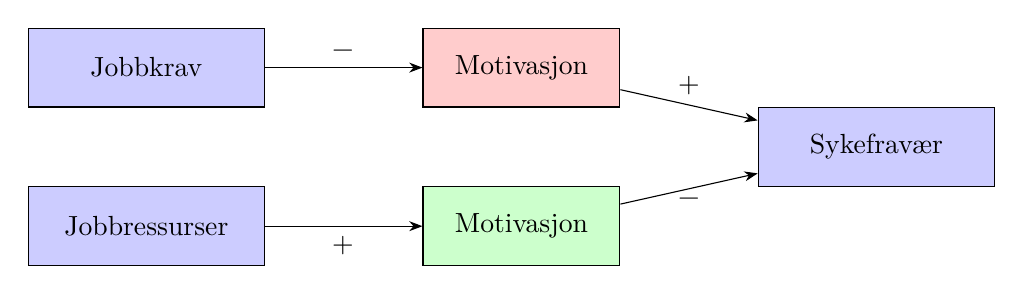
\begin{tikzpicture}[
      latent/.style={rectangle, draw, fill=blue!20, minimum width=3cm, minimum height=1cm},
      item/.style  ={rectangle, draw, fill=blue!10, font=\small},
      medi/.style  ={rectangle, draw, fill=green!20, minimum width=2.5cm, minimum height=1cm},
      medi2/.style ={rectangle, draw, fill=red!20,   minimum width=2.5cm, minimum height=1cm},
      moder/.style ={diamond,   draw, fill=yellow!20,aspect=2, minimum width=2.5cm, minimum height=1cm},
      >=Stealth,
      node distance=1cm and 2cm
    ]

    % Latente noder
    \node[latent]              (JK)  {Jobbkrav};
    \node[latent, below=of JK] (JR)  {Jobbressurser};

    % To separate motivasjons-noder
    \node[medi2, right=of JK] (M1) {Motivasjon};
    \node[medi,  right=of JR] (M2) {Motivasjon};

    % Piler fra latente til motivasjon med tegn
    \draw[->] (JK) -- node[midway, above] {$-$} (M1);
    \draw[->] (JR) -- node[midway, below] {$+$} (M2);

    % Sykefravær
    \node[latent, right=3cm of $(M1)!0.5!(M2)$] (SF) {Sykefravær};

    % Piler fra motivasjon til sykefravær med tegn
    \draw[->] (M1) -- node[midway, above] {$+$} (SF);
    \draw[->] (M2) -- node[midway, below] {$-$} (SF);

  \end{tikzpicture}
  \caption{JD–R-modellen}
  \label{fig:jdr_tikzz}
\end{figure}

Schaufeli \& Bakker (2004) testet i en SEM-modell hvordan jobbkrav og
jobbressurser forklarer utbrenthet og jobbengasjement. Studien viste at
utbrenthet og jobbengasjement var negativt korrelert, og at jobbkravene
hadde en positiv effekt på utbrenthet, mens jobbressursene hadde en
signifikant \textbf{positiv} effekt på jobbengasjement. Dette kan
understøtte at høye krav skaper stress og fravær, mens ressurser fremmer
engasjement og opplevelse av mestring. Mens denne studien fokuserer på
hvordan utbrenthet har en medierende effekt på forholdet mellom jobbkrav
og helseproblemer og engasjement medierer forholdet til jobbressurser og
intensjon om å slutte i arbeid. Studien deres inkluderte kun
respondenter fordelt på fire forskjellige arbeidsplasser og yrker, og vi
vil da videre fokusere på hvordan jobbkrav og jobbressurser påvirker
sykefravær gjennom motivasjon, og hvordan formue kan moderere disse
effektene for arbeidstakere i hele Norge.

\subsubsection{Formue som moderator}\label{sec-formue-jdr}

Vi mener at økonomiske ressurser som formue, kan hjelpe med å forklare
sykefraværet enda mer og vil bruke den som en ekstern modererende
faktor.

Hobfoll (1989) definerer jobbressurser som ressurser som kan hjelpe
individer med å håndtere jobbkrav og redusere stress. Formue kan ses på
som en form for jobbressurs, da den gir økonomisk trygghet og muligheter
for å håndtere jobbrelaterte utfordringer. Formue kan også bidra til å
redusere stress og øke trivsel, noe som igjen kan føre til lavere
sykefravær.

Formue gir en økonomisk buffer som kan redusere sårbarheten for
jobbrelatert stress. Personer med høy formue kan ha større valgfrihet i
arbeidslivet, og tåler lettere perioder med høy belastning uten at det
går like hardt utover helse eller jobbmotivasjon. Men personer med lav
eller negativ formue vil ofte være mer økonomisk avhengige av inntekten
fra arbeid, og kan derfor være mer sårbare for jobbrelatert stress

Formue kan også ha betydning for fremtidsperspektiv og indre motivasjon.
Personer med lav formue kan oppleve mindre kontroll over egen
livssituasjon og lavere forventninger til fremtidig økonomisk trygghet,
noe som potensielt svekker arbeidsglede og motivasjon.

Vi antar da at formue påvirker hvordan individet opplever og håndterer
jobbkrav og jobbressurser. Vi postulerer at formue fungerer som en
moderator for sensitiviteten til endringer i arbeidsforhold og inntekt.
En person med lav formue kan være mer sensitiv for både negative og
positive endringer i jobbkrav og jobbressurser siden den økonomiske
marginen er mindre. Motsatt kan en person med høy formue være mindre
sensitiv for endringer i jobbkrav og jobbressurser, og dermed oppleve
mindre stress og utbrenthet. Dette kan føre til at personer med høy
formue er mer motstandsdyktige mot negative effekter av jobbkrav og mer
mottakelige for positive effekter av jobbressurser. Dette kan bety at
effekten er ikke-lineær eller bue formet, hvor effekten er sterkest i de
med lavest formue og avtar med økende formue. Hvis det er
motivasjonsmessige effekter av formuenivå så kan det være at et lavt
formuenivå vil gjøre en mindre motivert og indirekte påvirke sykefravær,
men også fungere motsatt ved høy formue.

Denne antagelsen støttes av Üngüren et al. (2021) hvor de fant at
økonomisk velvære\footnote{Økonomisk velvære kan defineres som en
  tilstand der en person fullt ut kan møte nåværende og løpende
  økonomiske forpliktelser, kan føle seg trygg på sin økonomiske
  fremtid, og er i stand til å ta valg som gjør det mulig å nyte livet.
  Financial Protection Bureau) (2015)} fungerte som en moderator som
reduserte den negative effekten av jobbusikkerhet på utbrenthet blant
hotellansatte.

Ved å inkludere formue som en ekstern faktor i JD-R modellen, forsøker
vi å fange både den direkte effekten av økonomisk trygghet og hvordan
denne tryggheten forsterker eller demper effektene av jobbrelaterte
faktorer. I et samfunn med økende økonomisk ulikheter hvor forskjellen
mellom dem som har og dem som ikke har, blir større og større, er det
viktig å forstå hvordan dette påvirker arbeidstakere og deres helse.
Teoretisk i modellen vil formue da kunne forsterke effektene av
jobbressurser og fungere som en buffer mot jobbkrav, og dermed påvirke
sykefraværet.

\subsection{Tidligere forskning}\label{tidligere-forskning}

Tidligere empirisk forskning har over tid vist positive forhold mellom
forskjellige Job Demands-Resources-faktorer og årsaker som kan føre til
sykefravær.

\subsubsection{Mikronivå: JD-R-studier i helse- og
omsorgssektoren}\label{mikronivuxe5-jd-r-studier-i-helse--og-omsorgssektoren}

Vander Elst et al. (2016) utførte en JD-R med SEM-analyse på Belgisk
hjemmepleiepersonell. Jobbkrav og jobbressurser ble modellert som
prediktorer. Studien viste at jobbkravene var positivt assosiert med
utbrenthet, mens jobbressursene var positivt assosiert med
jobbengasjement. Denne studien viser også at JDR-mekanismer holder i
andre sammenhenger hvor arbeidstakere er under emosjonelt press og
skiftarbeid.

\subsubsection{Mikronivå:
formue-helse-koblinger}\label{mikronivuxe5-formue-helse-koblinger}

Jaeggi et al. (2021) undersøkte effekten av ulikhet i formue i et
småskala samfunn av innfødte i Tsimane i Bolivia med 871 observasjoner,
\(n = 871\). I studien testet de relativ husholdningrikdom og ulikhet i
formue mot forskjellige psykologiske variabler og helseutfall som
depresjon, BMI, blodtrykk og sykelighet.

Studien viste til en kobling mellom formueulikhet hvor de med lavere
formue hadde større sannsynlighet for å få høyere blodtrykk og
luftveissykdommer som kunne lede til dødsfall. De fant også at de med
høyere formue hadde lavere sannsynlighet for å få depresjon og høyere
BMI. Dette indikterer at ulikhet i formue kan moderere stress og
helserisiko på individnivå.

\subsubsection{Mikronivå: JD-R-studier i
Norge}\label{mikronivuxe5-jd-r-studier-i-norge}

Langseth-Eide \& Vittersø (2021) bygger videre på tidligere forskning og
adresserer limitasjonene ved Job Demands-Resources-modellen. De
argumenterer for at Job Demands-Resources-modellen ved tidligere
forskning har hatt fokus på organisasjonsnivået, og at det er viktig å
se på hvordan Job Demands-Resources-modellen kan brukes bedre på
jobbressurser, jobbengasjement og helserelaterte utfall. De gjorde en
paneldata studie på fast ansatte i Norge med to års tidsforsinkelse med
1533 ansatte første tidsperiode, \(n =1533\) og 1503 ansatte,
\(n = 1503\) neste tidsperiode.

Over lengre tid fant de at jobbressurser hadde en positiv effekt på
jobbengasjement, og at jobbengasjement var negativt assosiert med
sykefravær. Dette kan tyde på at høyere jobbressurser kan føre til
høyere jobbengasjement, som igjen kan føre til lavere sykefravær.

\subsubsection{Makronivå: Ulikhet i
samfunnet}\label{makronivuxe5-ulikhet-i-samfunnet}

JDR-modellen operer primært på individnivå, men en makroøkonomisk studie
om inntektsulikhet har vist at økonomisk ulikhet i en befolkning
korrelerer med høyere sykefravær og dårligere helse. Pickett \&
Wilkinson (2015) undersøkte sammenhengen mellom inntektsulikhet og helse
i 34 OECD-land, og fant at høyere inntektsulikhet var assosiert med
høyere sykefravær og dårligere helseutfall. Studien viste også at
inntektsulikhet hadde en negativ effekt på livskvalitet og trivsel, og
at dette kunne føre til økt sykefravær.

Mekanismene som følger på mikronivå er da:

\[
\text{Høyere jobbkrav} \rightarrow \text{Økt utbrenthet} \rightarrow \text{Høyere sykefravær} \rightarrow \text{Økt jobbengasjement} \rightarrow \text{Lavere sykefravær}
\]

Hvor formue fungerer som en moderator ved å påvirke stress til individer
før jobbkravene utløser negative effekter på helse.

På makronivå vil samfunnsmessig ulikhet forme de jobbkrav og ressurser
som virksomheter og arbeidstakere får, og dermed styrke JDR-mekanismer,
også på tvers av sektorer og bransjer. Dermed får vi et teoretisk og
empirisk grunnlag for vår undersøkelse av at:

\[
\text{Formue} \rightarrow \text{Jobbkrav og jobbressurser} \rightarrow \text{Sykefravær i Norge}
\]

\subsection{Modelloppsett}\label{modelloppsett}

Modellen vi blir å bruke blir da som følger:

\begin{figure}
  \centering
  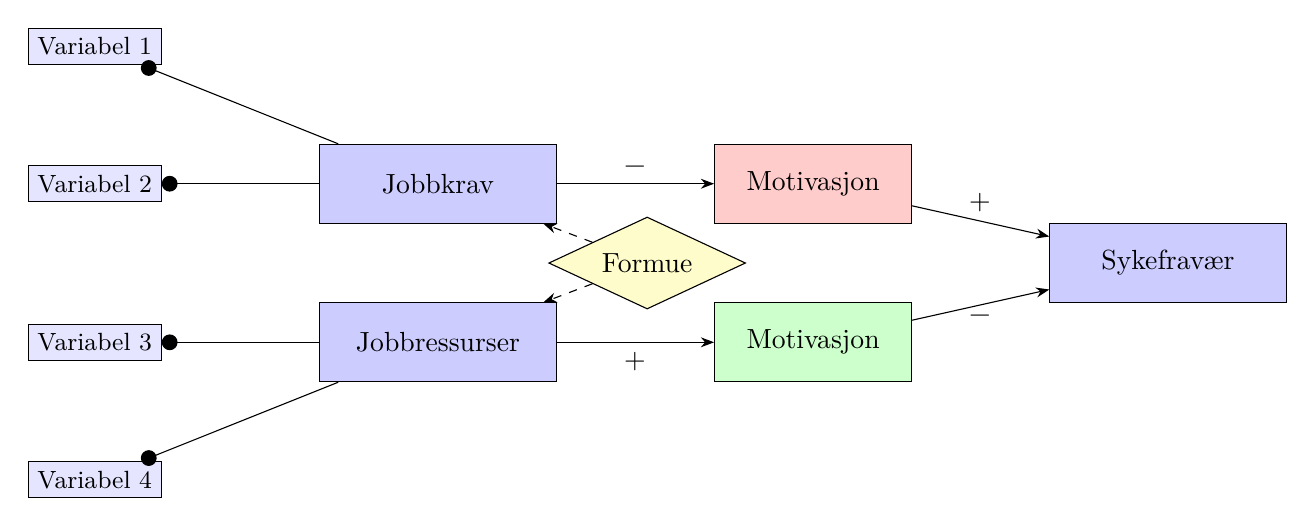
\begin{tikzpicture}[
      latent/.style={rectangle, draw, fill=blue!20, minimum width=3cm, minimum height=1cm},
      item/.style  ={rectangle, draw, fill=blue!10, font=\small},
      medi/.style  ={rectangle, draw, fill=green!20, minimum width=2.5cm, minimum height=1cm},
      medi2/.style ={rectangle, draw, fill=red!20,   minimum width=2.5cm, minimum height=1cm},
      moder/.style ={diamond,   draw, fill=yellow!20,aspect=2, minimum width=2.5cm, minimum height=1cm},
      >=Stealth,
      node distance=1cm and 2cm
    ]

    % Latente noder
    \node[latent]              (JK)  {Jobbkrav};
    \node[latent, below=of JK] (JR)  {Jobbressurser};

    % Indikator-noder for Jobbkrav
    \node[item, above left=of JK] (v1) {Variabel 1};
    \node[item, left=of JK]       (v2) {Variabel 2};
    \draw[-{Circle[length=2mm]}] (JK) -- (v1);
    \draw[-{Circle[length=2mm]}] (JK) -- (v2);

    % Indikator-noder for Jobbressurser
    \node[item, left=of JR]        (v3) {Variabel 3};
    \node[item, below left=of JR]  (v4) {Variabel 4};
    \draw[-{Circle[length=2mm]}] (JR) -- (v3);
    \draw[-{Circle[length=2mm]}] (JR) -- (v4);

    % Moderator-node plassert midt over
    \node[moder, right=1.4cm of $(JK)!0.5!(JR)$] (FN) {Formue};
    \draw[->, dashed] (FN) -- (JK);
    \draw[->, dashed] (FN) -- (JR);

    % To separate motivasjons-noder
    \node[medi2, right=of JK] (M1) {Motivasjon};
    \node[medi,  right=of JR] (M2) {Motivasjon};

    % Piler fra latente til motivasjon med tegn
    \draw[->] (JK) -- node[midway, above] {$-$} (M1);
    \draw[->] (JR) -- node[midway, below] {$+$} (M2);

    % Sykefravær
    \node[latent, right=3cm of $(M1)!0.5!(M2)$] (SF) {Sykefravær};

    % Piler fra motivasjon til sykefravær med tegn
    \draw[->] (M1) -- node[midway, above] {$+$} (SF);
    \draw[->] (M2) -- node[midway, below] {$-$} (SF);

  \end{tikzpicture}
  \caption{Utvidet JD–R-modell med formue som moderator og separate motivasjonsløp.}
  \label{fig:jdr_tikz}
\end{figure}

I modellen vår (\autoref{fig:jdr_tikz}) har vi inkludert formue som en
moderator som påvirker både jobbkrav og jobbressurser. Dette betyr at
formue kan endre hvordan jobbkrav og jobbressurser påvirker
sykefraværet. Vi har også separate motivasjonsløp for jobbkrav og
jobbressurser, som gjør at vi kan se hvordan motivasjon påvirkes av
begge disse faktorene. Vi antar at formuen blir å fungere som en
stress-avlastning eller buffer mot jobbkravene og forsterke effekten av
jobbressurser, og fungere som en psykologisk trygghet. Dette kan føre
til at personer med høyere formue opplever lavere sykefravær, mens de
med lavere formue kan oppleve høyere sykefravær på grunn av økt stress
og lavere tilgang til ressurser.

\subsubsection{Hovedmodell for sykefravær
(SF)}\label{hovedmodell-for-sykefravuxe6r-sf}

Vi antar at sykefraværet (SF) i hovedsak påvirkes av:

Jobbkrav (JK) (effekten av arbeidsbelastning),

Motivasjon (M) (som en mekanisme/medierende faktor),

Formuenivå (FN) (som hovedprediktor og også direkte påvirker SF),

Så kan vi ha en X som er en mengde kontrollvariabler som for eksempel
avtalte dager, demografi, arbeidsrelaterte forhold osv.

\[
SF_i = \beta_0 + \beta_1 JK_i + \beta_2 M_i + \beta_3 FN_i + \Sigma_j \beta_{4j}X_{ij} + \epsilon_{1i}
\]

Der \(i\) er individet, \(\beta_0\) er konstanten, \(\beta_1\),
\(\beta_2\), \(\beta_3\) er koeffisientene for henholdsvis jobbkrav,
motivasjon og formuenivå, \(\Sigma_j \beta_{4j}X_{ij}\) fanger opp
effekter av eventuelle kontrollvariabler, \(\epsilon_{1i}\) er
feilleddet.

Denne likningen innebærer at formuenivået ikke bare antas å ha en
direkte effekt på sykefravær, men via motivasjon så kan effekten også gå
via en indirekte kanal.

\subsubsection{Ligning for motivasjon
(M)}\label{ligning-for-motivasjon-m}

Motivasjonen antas å bli påvirket av:

Jobbressurser (JR) (dvs. støtte og autonomi i arbeidet),

Formuenivå (FN) (som antas å påvirke hvor sensitiv man er for endringer
i inntekt -- dvs. hvordan man prioriterer fritid/arbeid),

X er kontrollvariabler som f.eks. utdanning eller andre relevante
demografiske/yrkesmessige mål.

\[
M_i = \alpha_0 + \alpha_1 JR_i + \alpha_2 FN_i + \Sigma_k \alpha_{3k}X_{ik} + \epsilon_{2i}
\]

Der \(\alpha_0\) er konstanten, \(\alpha_1\) og \(\alpha_2\) er
koeffisientene for henholdsvis jobbressurser og formuenivå,
\(\Sigma_k \alpha_{3k}X_{ik}\) fanger opp effekter av eventuelle
kontrollvariabler, \(\epsilon_{2i}\) er feilleddet.

putter inn utdanning og alder i x.

Er nokk forskjell på sykefravær på alder ung/gammel. hvor stor forskjell
mellom de på ung og gammel basert på formue

\section{Metode og data}\label{metode-og-data}

I dette kapitlet går vi gjennom datagrunnlag og metode for oppgaven. Vi
vil først forklare hvordan dataene er fremskaffet, så forklare
variablene, og til slutt forklare metoden. Vi vil også gi en innledende
oversikt over dataene, inkludert deskriptiv statistikk for alle
variablene i analysen.

I problemstillingen \emph{forklarer nivået på formue sykefraværet i
Norge?} så velger vi å bruke en Structural Equation Model fordi denne
kan bedre vise oss på hvilken måte formue påvirker sykefraværet og om
det finnes noen indirekte sammenhenger mellom variablene vi velger å
bruke, dette gjør analysen mer kompleks, men vi kan bedre peke direkte
på hvilke effekter som er positive eller negative på selve sykefraværet.

\subsection{Data}\label{data}

Dataen vi bruker er hentet fra Statistisk sentralbyrå (SSB) sin
\href{https://www.ssb.no/arbeid-og-lonn/arbeidsmiljo-sykefravaer-og-arbeidskonflikter/artikler/levekarsundersokelsen-om-arbeidsmiljo-2022}{levekårsundersøkelse
om arbeidsmiljø}, som ble gjennomført i 2022. Vedlagt følger et bilde av
kodeboken:

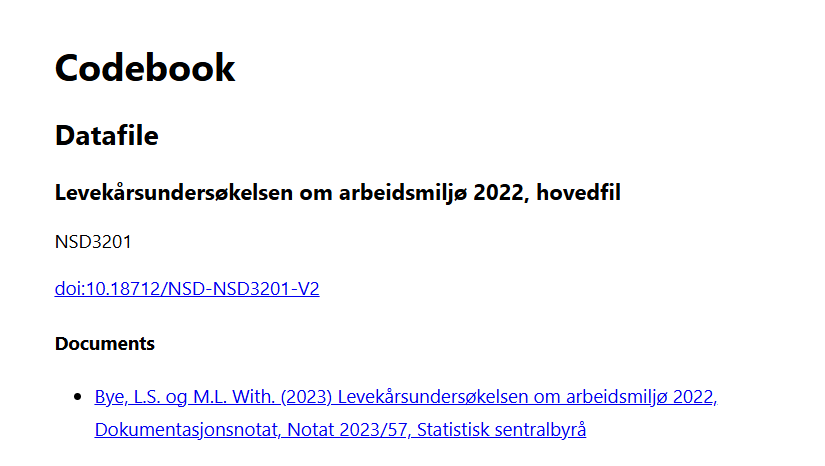
\includegraphics{dokumentobjekter/bilder/codebook.png}

Statistisk sentralbyrå har gjennomført levekårsundersøkelser siden 1973.
Levekårsundersøkelsen kartlegger arbeidsmiljøforhold blant sysselsatte i
Norge, og tar opp temaer som forhold på arbeidsplassen, fysisk,
ergonomisk og psykososialt arbeidsmiljø, yrkesrelaterte helseplager og
sykefravær og krav og muligheter for selvbestemmelse på jobb.

\subsection{Datakilde og utvalg}\label{datakilde-og-utvalg}

Undersøkelsen er basert på et landsrepresentativt utvalg på 35 345
sysselsatte personer i alderen 18-66 til undersøkelsen i 2022. Utvalget
er tilfeldig trukket fra folkeregisteret, og dataene er samlet inn
gjennom telefonintervjuer og selvadministrert webskjema fra august 2022
til april 2023.

Den totale svarprosenten for undersøkelsen var på 51 prosent, og dataene
er vektet for å være representativt for den norske befolkningen i
alderen 18-66 for å korrigere for noen av skjevhetene i forbindelse med
frafall.

\subsection{Variabler}\label{variabler}

Vi kommer til å bruke flere variabler fra levekårsundersøkelsen for å
analysere sammenhengen mellom formue og sykefravær. Vi vil bruke både
avhengige og uavhengige variabler, latente\footnote{En latent varibel er
  et underliggende, uobserverbart konstrukt som ikke kan måles direkte,
  men som modelleres gjennom flere målbare indikatorer. I SEM tolkes for
  eksempel «motivasjon», «jobbkrav» og «jobbressurser» som latente
  variabler: vi antar at variasjonen i et sett av attestspørsmål
  (indikatorer) reflekterer den samme underliggende faktoren.}
variabler, samt kontrollvariabler for å kontrollere for andre faktorer
som kan påvirke sykefraværet.

\subsubsection{Avhengig og uavhengig
hovedvariabel}\label{avhengig-og-uavhengig-hovedvariabel}

Sykefravær:

Datasettet inneholder en ferdig variabel for sykefraværsprosent
(sfpros\_uten\_feriekorr\_2022, sfpros\_uten\_feriekorr\_2023), men vi
velger å beregne denne selv for å ha med egenmeldings dager, også for å
kunne ta høyde for avtalt arbeidstid.

Vi benytter variablene sfdagsvj\_2022 (sykefraværsdagsverk) og
mdagsv\_2022 (avtalte dagsverk) fra Levekårsundersøkelsen.
Sykefraværsprosenten \((SF_i)\) for individ \(i\) er da
sykefraværsdagsverk delt på avtalte dagsverk for hvert individ.

Formue:

Bruttofinanskapital i alt (BF) vil være vår hoveduavhengige variabel, og
vi vil bruke bruttofinanskapital i alt som mål på formue. Denne
variabelen inneholder verdien av alle finansielle eiendeler som
respondenten eier, inkludert kontanter, aksjer, obligasjoner og andre
investeringer og har en maks verdi på 2 500 000.

Vi vil dele denne inn i tre forskjellige tertiler \footnote{Tertiler er
  en statistisk metode for å dele opp et datasett i tre like store
  deler, slik at hver del inneholder en tredjedel av observasjonene.}
for formuegrupper: 0 - 43 333.33, 43 333.33 - 200 000 og 200 000 - 2 500
000. Dette vil gi oss mulighet til å se om det er forskjeller i
sykefravær mellom de forskjellige tertilene. Vi definerer de som lav,
middels og høy formue. Vi vil også bruke log-transformasjon av formue
for å se om det er noen forskjeller i sykefravær mellom de forskjellige
tertilene. Dette kan være nyttig for å se om det er noen ikke-lineære
sammenhenger mellom formue og sykefravær, og for å håndtere høy skjevhet
i dataene, ettersom de fleste har lav formue og få har høy formue.

Vi tror formue spiller inn til hvor sensitiv du er til endringer i
inntekt. Altså ditt konsumnnivå eller etterspurt fritid endrer seg ulikt
basert på om du har mye formue eller ikke. Dette kan være fordi du har
mer buffer til å tåle endringer i inntekt, og dermed kan du være mer
villig til å ta deg fri fra jobb. Og motsatt om du har lite formue så
vil du være mer sensitiv til endringer i inntekt, og dermed vil du være
mer villig til å jobbe mer for å opprettholde inntekten din. Dette kan
føre til at de med høyere formue har lavere sykefravær, mens de med
lavere formue har høyere sykefravær.

\subsubsection{Kontrollvariabler}\label{kontrollvariabler}

Alder:

Alder til respondenten ved utgangen av 2022. Denne kontrollvariabelen
gjør vi ordinal ettersom vi fordeler alderen til respondenten i
aldersgrupper. Vi vil bruke aldersgruppene 18-29, 30-39, 40-49, 50-59 og
60-66 år. Da kan vi påpeke hvis det er forskjeller i sykefravær mellom
de forskjellige aldersgruppene fra unge til eldre personer.

Kjønn:

Kjønn til respondenten. Denne kontrollvariabelen er en dummyvariabel,
hvor 0 er kvinne og referansekategorien 1 er menn. Da vil vi i analysen
direkte se effekten av å være kvinne på sykefraværet.

Utdanning:

Utdanningsnivået til respondenten er en ordinal variabel, og vi vil
bruke utdanningsgruppene grunnskole eller mindre, videregående skole,
Universitet/Høgskole og forskernivå. Vi vil bruke denne variabelen for å
kontrollere for eventuelle utdanningsforskjeller i sykefraværet.

Tilfredshet med arbeid:

Selvrapportert tilfredshet med arbeid (TS) er en ordinal variabel, og vi
vil bruke denne variabelen for å kontrollere for eventuelle forskjeller
i sykefraværet basert på hvor tilfreds respondenten er med jobben sin.
Denne variabelen er målt på en skala fra 1 til 10, hvor 1 er svært
misfornøyd og 10 er svært fornøyd.

Motivasjon:

For variabelen motivasjon bruker vi selvrapportert motivasjon på jobb
(M) som en ordinal variabel, og vi vil bruke denne variabelen for å
kontrollere for eventuelle forskjeller i sykefraværet basert på hvor
motivert respondenten er på jobben sin. Denne variabelen er målt på en
skala fra 1 til 10, hvor 1 er svært lite motivert og 10 er svært
motivert.

Barn:

Antall barn under 18 år i husholdningen som er en kontinuerlig variabel.
Vi vil bruke denne variabelen for å kontrollere for eventuelle
forskjeller i sykefraværet basert på hvor mange barn respondenten har.

Vi vil også mulig bruke dummyvariabler for å kontrollere for andre
faktorer som kan påvirke sykefraværet, som for eksempel yrke, bransje og
arbeidsforhold.

\subsection{Deskriptiv statistikk}\label{deskriptiv-statistikk}

I dette avsnittet vil vi gi en oversikt over deskriptiv statistikk for
alle variablene i analysen. Vi vil presentere gjennomsnitt,
standardavvik og minimums- og maksimumsverdier for alle variablene, samt
korrelasjonsmatrisen for de uavhengige variablene.

I \autoref{tab:deskriptiv} presenteres deskriptiv statistikk for alle
variablene i analysen. Vi ser at sykefraværet i 2022 har et gjennomsnitt
på 12.27 prosent, med et standardavvik på 13.49 prosent. Alder har et
gjennomsnitt på 42.80 år, med et standardavvik på 12.28 år.
Utdanningsnivået har et gjennomsnitt på 4.38, som tilsvarer videregående
skole, med et standardavvik på 1.23.

Av de opprinnelig 17971 inviterte respondentene i datasettet så
fullførte kun 2 080 svarene til alle de relevante variablene. Hvor
eksakt responsrate da blir \(\frac{2080}{17971} = 11.6\%\). Dette kan
føre til skjevheter i dataene, og kan bli en svakhet ved analysen når vi
tolker resultatene. Siden det er vanskelig for oss å vite om det er
systematiske forskjeller mellom de som svarte og de som ikke svarte, så
kan vi ikke si noe sikkert om hvor representativt utvalget er for den
norske befolkningen. Vi blir å sammenlikne alder og kjønn i datasettet
med SSB sine tall for å se om det er noen forskjeller, samt teste
gjennomsnittsalder, og gjennomsnittlig sykefravær for de som svarte og
de som ikke svarte. Hvis det er store forskjeller blir vi å måtte bruke
vektjustering for å korrigere for skjevhetene i dataene.

\begin{table}[ht]
\centering
\begin{tabular}{lrrrrrrr}
\toprule
Variabel & Min & 1.\,Q & Median & Mean & 3.\,Q & Max & N \\
\midrule
Sykefravær 2022                 &   0 &   3 &   7 & 12.27 &  16 &  92 & 2080 \\
Alder                            &  18 &  32 &  43 & 42.80 &  53 &  66 & 2080 \\
Utdanning                        &   2 &   4 &   4 &  4.38 &   6 &   8 & 2080 \\
Kjønn (1=Mann, 2=Kvinne)         &   1 &   1 &   2 &  1.63 &   2 &   2 & 2080 \\
Tilfredshet                      &   1 &   1 &   2 &  2.05 &   3 &   8 & 2080 \\
Motivasjon                       &   1 &   1 &   2 &  2.16 &   3 &   9 & 2080 \\
Barn                             &   0 &   0 &   0 &  0.15 &   0 &   1 & 2080 \\
Støtte fra sjef                  &   1 &   1 &   2 &  2.25 &   3 &   9 & 2080 \\
Støtte fra kollega               &   1 &   1 &   2 &  1.81 &   2 &   9 & 2080 \\
Tilbakemelding fra sjef          &   1 &   2 &   3 &  3.05 &   4 &   9 & 2080 \\
Arbeidsresultater                &   1 &   2 &   2 &  2.59 &   3 &   9 & 2080 \\
Selvbestemmelse (oppgaver)       &   1 &   3 &   3 &  3.25 &   4 &   9 & 2080 \\
Selvbestemmelse (arbeidsinnhold) &   1 &   2 &   2 &  2.48 &   3 &   9 & 2080 \\
Grad arbeidstempo                &   1 &   2 &   3 &  2.87 &   4 &   8 & 2080 \\
Påvirkningsgrad                  &   1 &   2 &   3 &  2.75 &   3 &   9 & 2080 \\
For mye arbeid                   &   1 &   1 &   2 &  1.94 &   2 &   8 & 2080 \\
Høyt arbeidstempo                &   1 &   1 &   2 &  1.78 &   2 &   9 & 2080 \\
Ekstra arbeid                    &   1 &   2 &   4 &  3.43 &   5 &   9 & 2080 \\
\bottomrule
\end{tabular}
\caption{Deskriptiv statistikk for hovedvariabler (N = 2080)}
\label{tab:deskriptiv}
\end{table}

I \autoref{tab:deskr_formue} presenteres deskriptiv statistikk for
sykefravær, alder, motivasjon og tilfredshet etter formuegruppe. Vi ser
at sykefraværet i 2022 har et gjennomsnitt på 12.72 prosent for de med
lav formue, 12.00 prosent for de med middels formue og 12.09 prosent for
de med høy formue. Dette tyder på at det ikke er noen store forskjeller
i sykefraværet mellom de forskjellige formuegruppene. Vi ser også at det
er små forskjeller i alder mellom de forskjellige formuegruppene, der de
med høy formue er eldre enn de med lav og middels formue. Dette kan vise
oss at det er en sammenheng mellom alder og formue, der eldre personer
har høyere formue enn yngre personer.

Motivasjonen er også høyere for de med lav formue enn de med høy formue,
noe som kan si at de med lav formue er mer motivert enn de med høy
formue. Dette kan være fordi de med lav formue har mer å jobbe for, og
derfor er mer motivert til å jobbe hardt. Tilfredsheten er også høyere
for de med lav formue enn de med høy formue, men det er generelt små
forskjeller i tilfredsheten mellom de forskjellige formuegruppene.

\begin{table}[ht]
\centering
\begin{tabular}{lcccccc}
\toprule
 & \multicolumn{2}{c}{Lav formue (n=705)} 
 & \multicolumn{2}{c}{Middels formue (n=704)} 
 & \multicolumn{2}{c}{Høy formue (n=719)} \\
\cmidrule(r){2-3}\cmidrule(lr){4-5}\cmidrule(l){6-7}
Variabel            & M     & SD    & M     & SD    & M     & SD    \\
\midrule
Alder               & 40.72 & 12.28 & 41.67 & 11.81 & 45.94 & 12.07 \\
Motivasjon          &  2.18 &  1.03 &  2.23 &  1.03 &  2.08 &  0.95 \\
Sykefravær 2022     & 12.72 & 13.49 & 12.00 & 14.83 & 12.09 & 14.26 \\
Tilfredshet         &  2.11 &  0.97 &  2.08 &  0.90 &  1.98 &  0.90 \\
\bottomrule
\end{tabular}
\caption{Deskriptiv statistikk etter formuegruppe}
\label{tab:deskr_formue}
\end{table}

I \autoref{tab:deskr_kjonn} presenteres deskriptiv statistikk for
sykefravær etter kjønn. Vi ser at sykefraværet i 2022 har et
gjennomsnitt på 10.92 prosent for menn og 13.06 prosent for kvinner,
kvinner har også høyere sykefravær enn menn. Dette kan skyldes at
kvinner i større grad enn menn jobber i yrker med høyere sykefravær,
eller at kvinner er mer tilbøyelige til å rapportere sykefravær enn
menn. Det kan også være andre faktorer som påvirker sykefraværet, som
for eksempel alder, utdanning og arbeidsforhold. Vi ser også at vi har
en overvekt av kvinner i utvalget, der 63.1 prosent av respondentene er
kvinner og 36.9 prosent er menn. Dette viser oss at det er en skjevhet i
utvalget, der kvinner er overrepresentert i forhold til menn.

\begin{table}[ht]
\centering
\begin{tabular}{lrrrr}
\toprule
Kjønn   & N   & \%   & Gj.snitt sykefravær & SD    \\
\midrule
Mann    & 785 & 36.9 & 10.92               & 13.04 \\
Kvinne  & 1343 & 63.1 & 13.06               & 14.79 \\
\bottomrule
\end{tabular}
\caption{Deskriptiv statistikk for sykefravær etter kjønn (N = 2 128)}
\label{tab:deskr_kjonn}
\end{table}

I \autoref{tab:deskr_utdanning} presenteres deskriptiv statistikk for
sykefravær etter utdanningsnivå. Vi ser at sykefraværet i 2022 har et
gjennomsnitt på 12.82 prosent for de med grunnskole eller mindre, 12.46
prosent for de med videregående skole og 11.67 prosent for de med
universitet/høgskole. Dette tyder på at sykefraværet er høyere for de
med lavere utdanning, og at det kan være er en sammenheng mellom
utdanningsnivå og sykefravær.

\begin{table}[ht]
\centering
\begin{tabular}{lrrrr}
\toprule
Utdanningsnivå                & N   & \%   & Gj.snitt sykefravær & SD    \\
\midrule
Grunnskole eller mindre       & 369 & 17.3 & 12.82               & 15.56 \\
Videregående                   &1074 & 50.5 & 12.46               & 14.26 \\
Universitet/Høgskole           & 685 & 32.2 & 11.67               & 13.31 \\
\bottomrule
\end{tabular}
\caption{Deskriptiv statistikk for sykefravær i 2022 etter utdanningsnivå (N = 2 128).}
\label{tab:deskr_utdanning}
\end{table}

I \autoref{fig:histogram} presenteres histogram og tetthetskurve for
sykefraværet i 2022. Vi ser at sykefraværet er høyreskjevt, med en
høyere andel av respondentene som har lavt sykefravær enn de som har
høyt sykefravær både på menn og kvinner. Vi vet fra
\autoref{tab:deskr_kjonn} at gjennomsnittet for begge kjønn er på
omtrent 11 prosent for menn mens det er på 13 prosent for kvinner, noe
som gjenspeiles i grafen. Det er vanskelig å se, men det er også noen
uteliggere hvor flere respondenter har mer enn 40 prosent sykefravær på
både menn og kvinner.

\begin{figure}[H]
\caption{Histogram og tetthetskurve for sykefravær i 2022}
\label{fig:histogram}
\centering
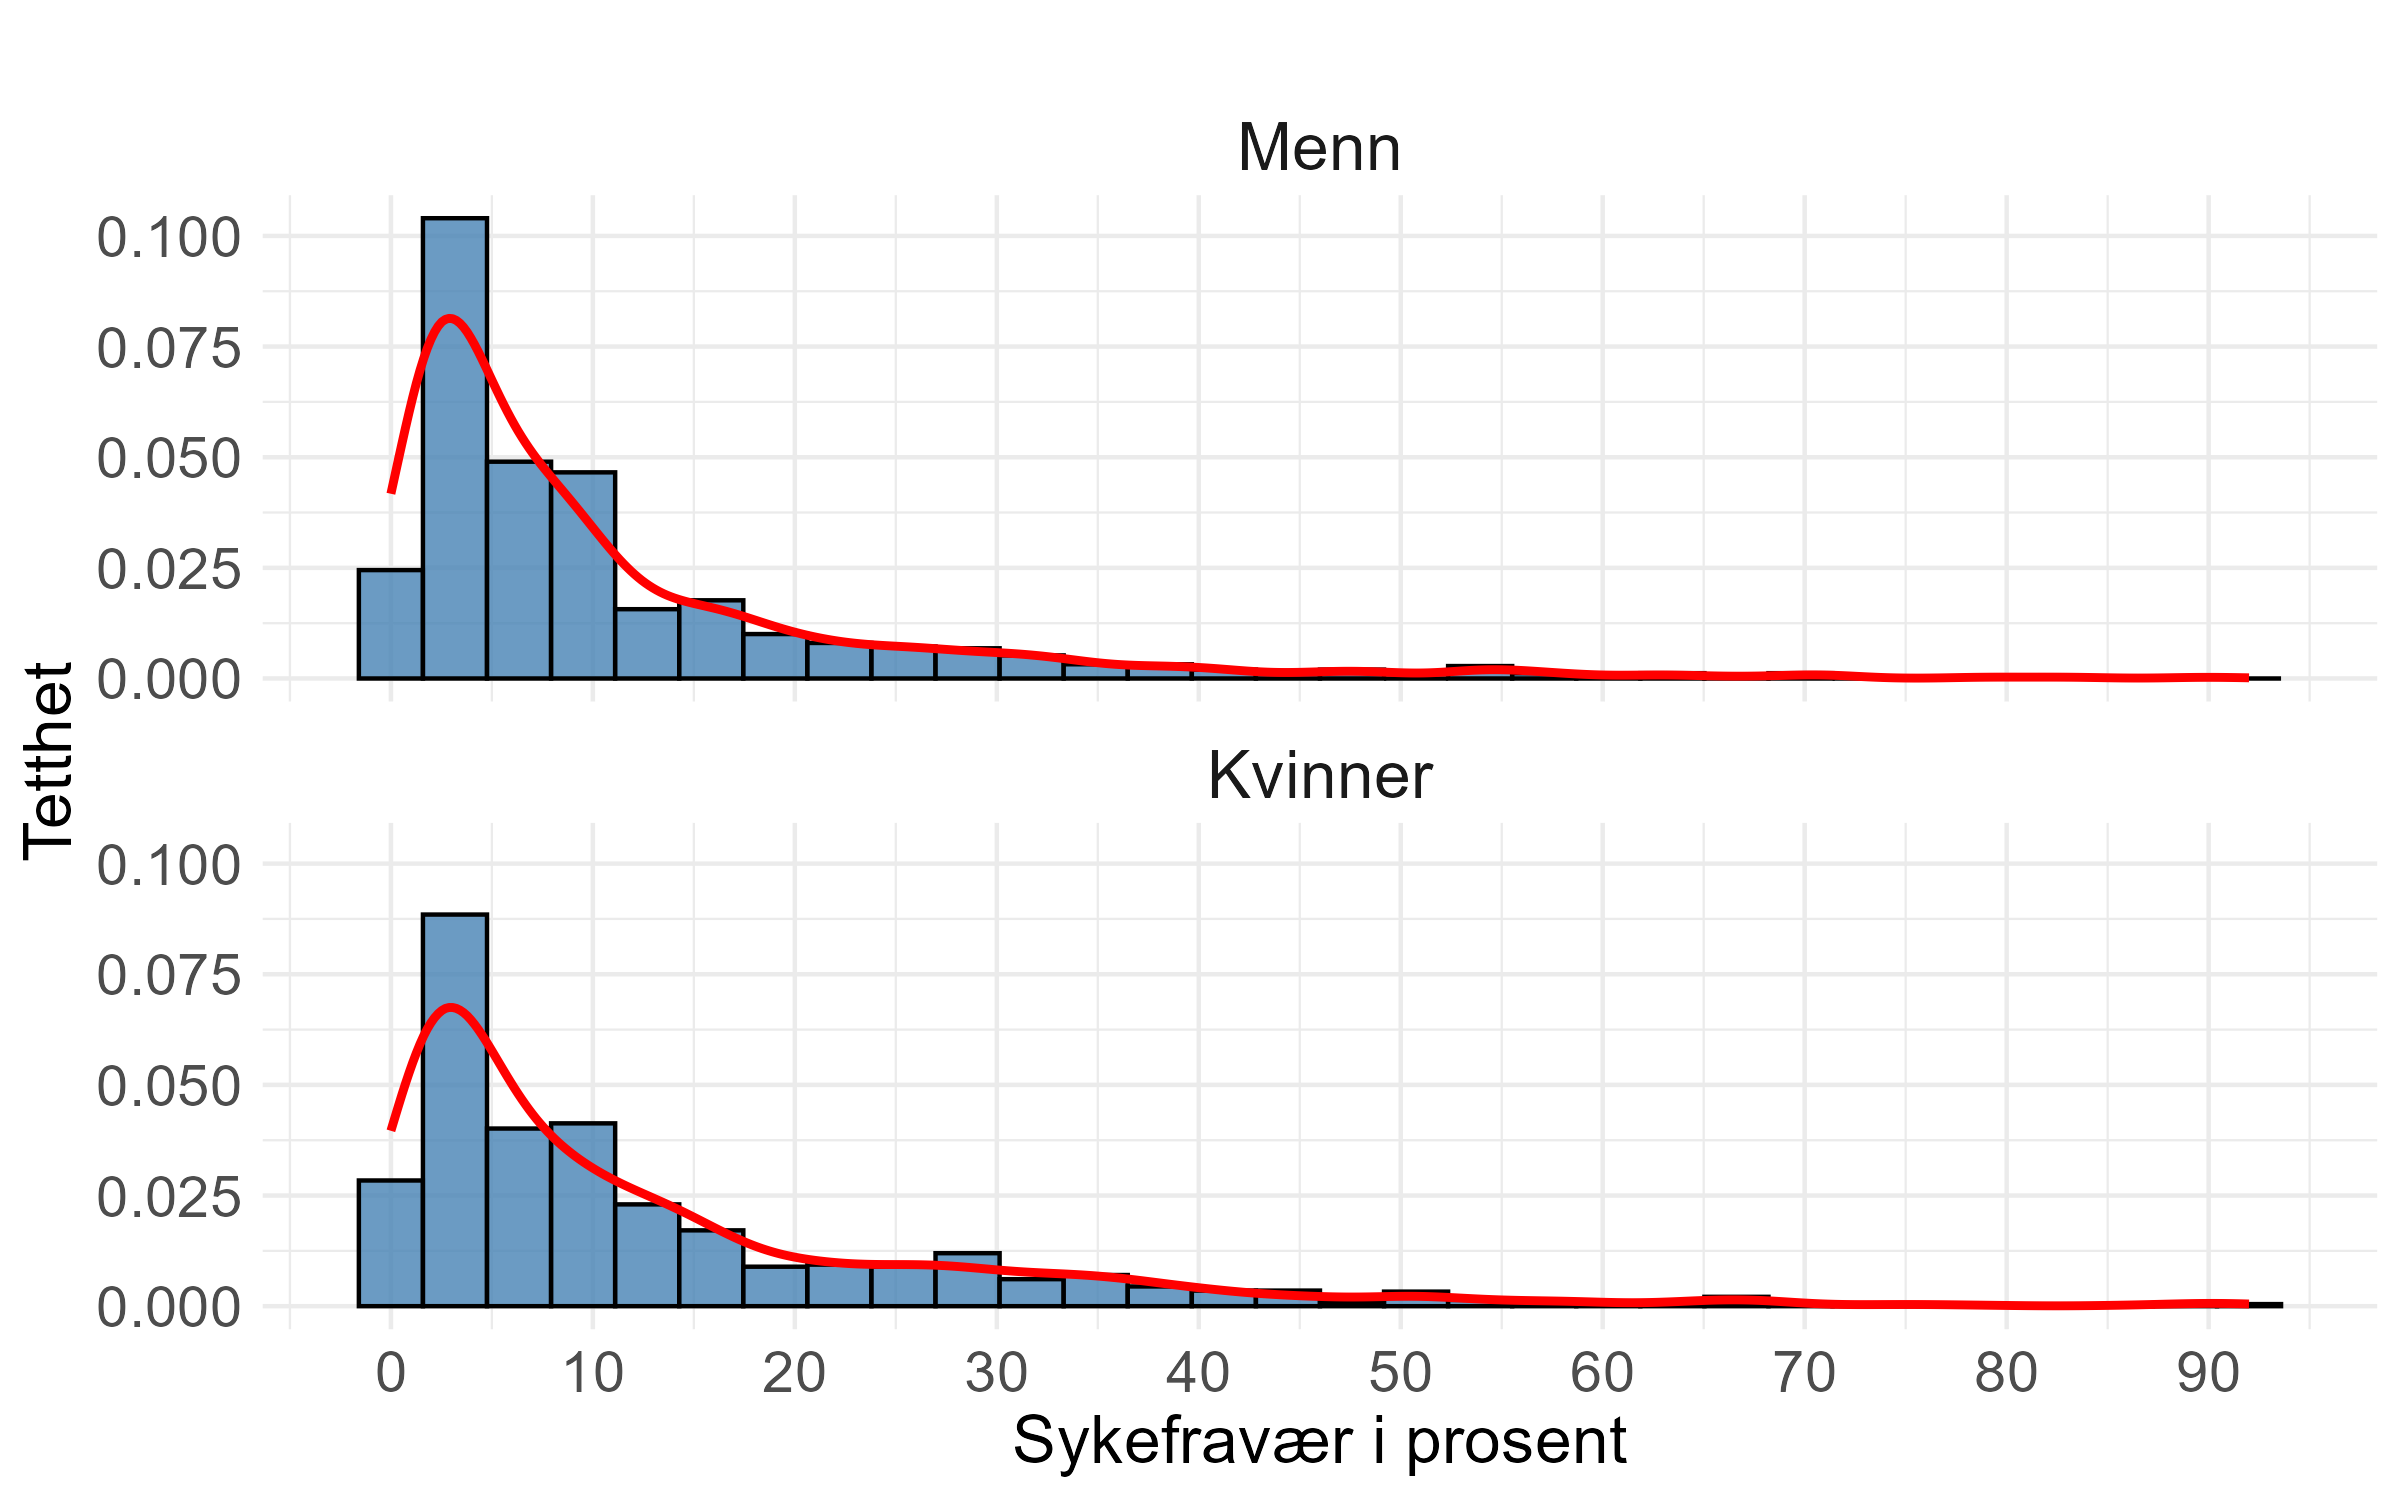
\includegraphics[width=0.8\textwidth]{dokumentobjekter/figurer/fig_1.png}
\end{figure}

Når vi ser på aldersfordelingen i \autoref{fig:histogram} så ser vi at
den er jevn og symmetrisk fordelt blant respondentene. Som nevnt
tidligere så er spennet på alderene til respondentene i undersøkelsen
mellom 18 til 66 år. Medianalderen kan man se i den blå stiplede linjen
som er på 43 år for menn og 44 år for kvinner.

\begin{figure}[H]
\caption{Histogram og tetthetskurve for alder}
\label{fig:histogram}
\centering
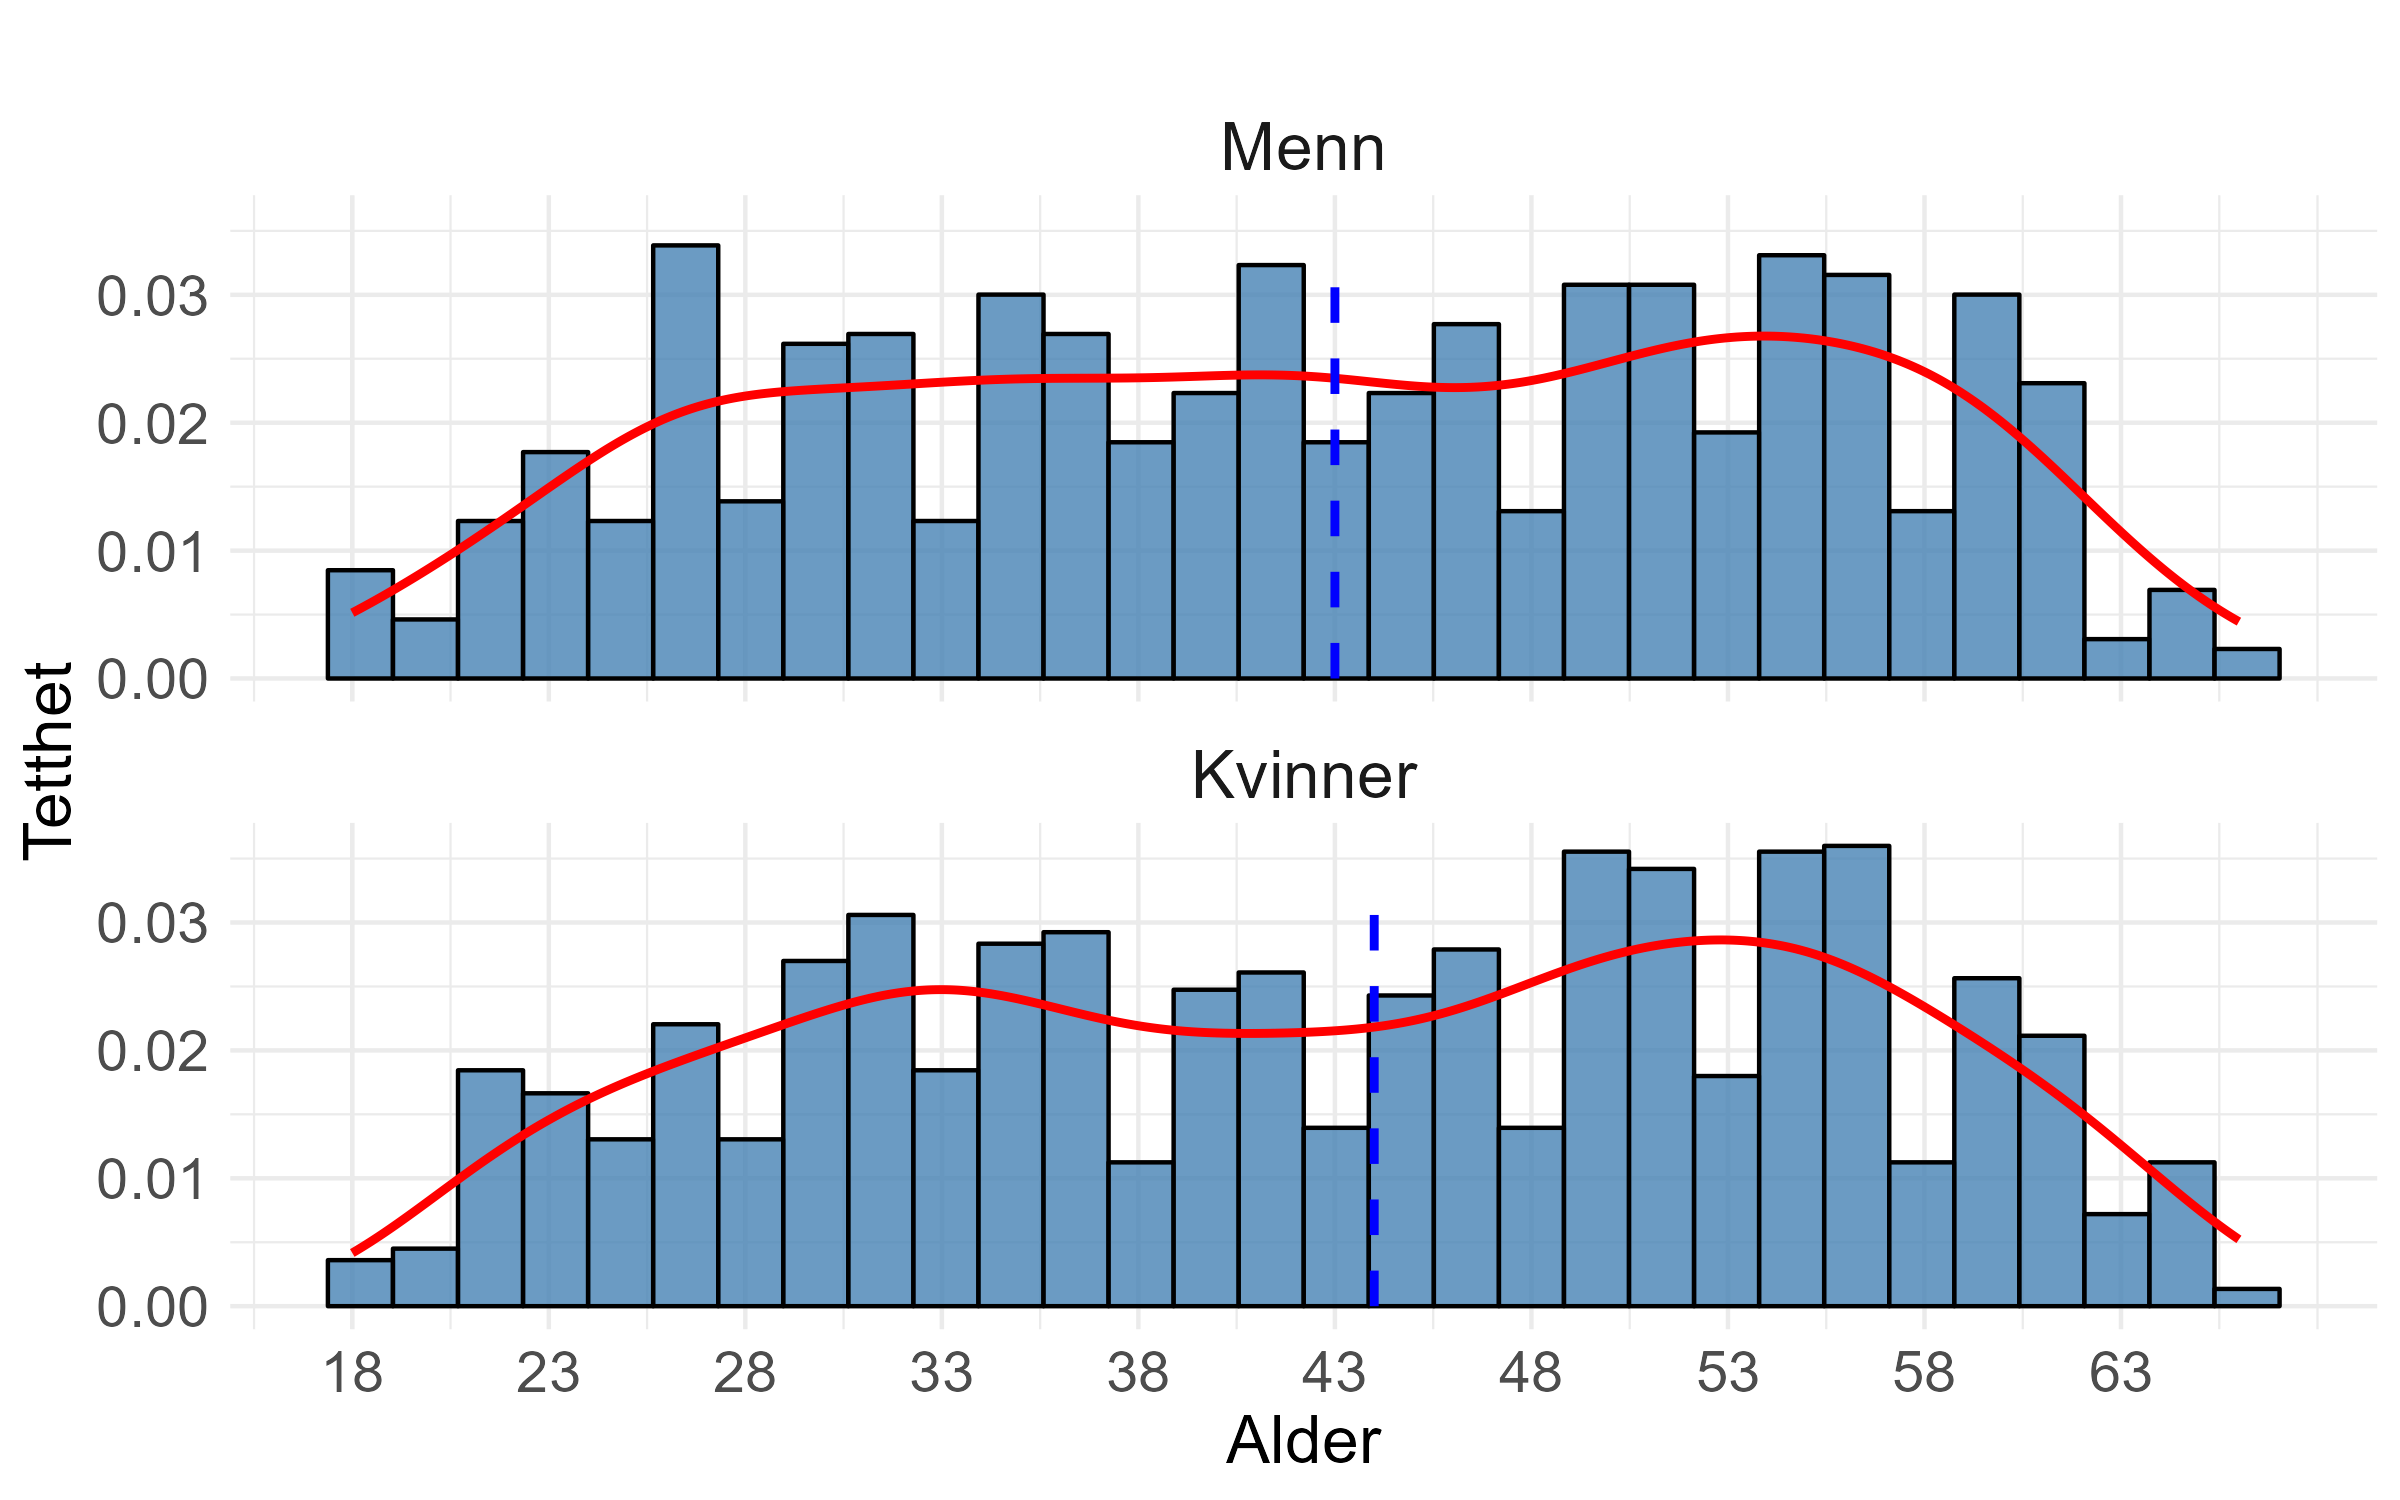
\includegraphics[width=0.8\textwidth]{dokumentobjekter/figurer/fig_2.png}
\end{figure}

For analysen så har vi fordelt alder inn i breddeintervaller på omtrent
10 år, og aldersgruppene er delt inn i 18-29, 30-39, 40-49, 50-59 og
60-66 år. I \autoref{fig:barplot} presenteres et barplot av
aldersgruppene. Vi ser at det er flest respondenter i aldersgruppen
50-59 år med 27.4 prosent, og at det er færrest respondenter i
aldersgruppen 60-66 år med 8.3 prosent. Dette fordi det er aldersgruppen
som er fordelt inn i det laveste breddeintervallet. Ellers er det jevnt
fordelt mellom de andre aldersgruppene, der aldersgruppen 40-49 år har
22.7 prosent, aldersgruppen 30-39 år har 23.5 prosent og aldersgruppen
18-29 år har 17.9 prosent.

\begin{figure}[H]
\caption{Aldersgruppefordeling}
\label{fig:barplot}
\centering
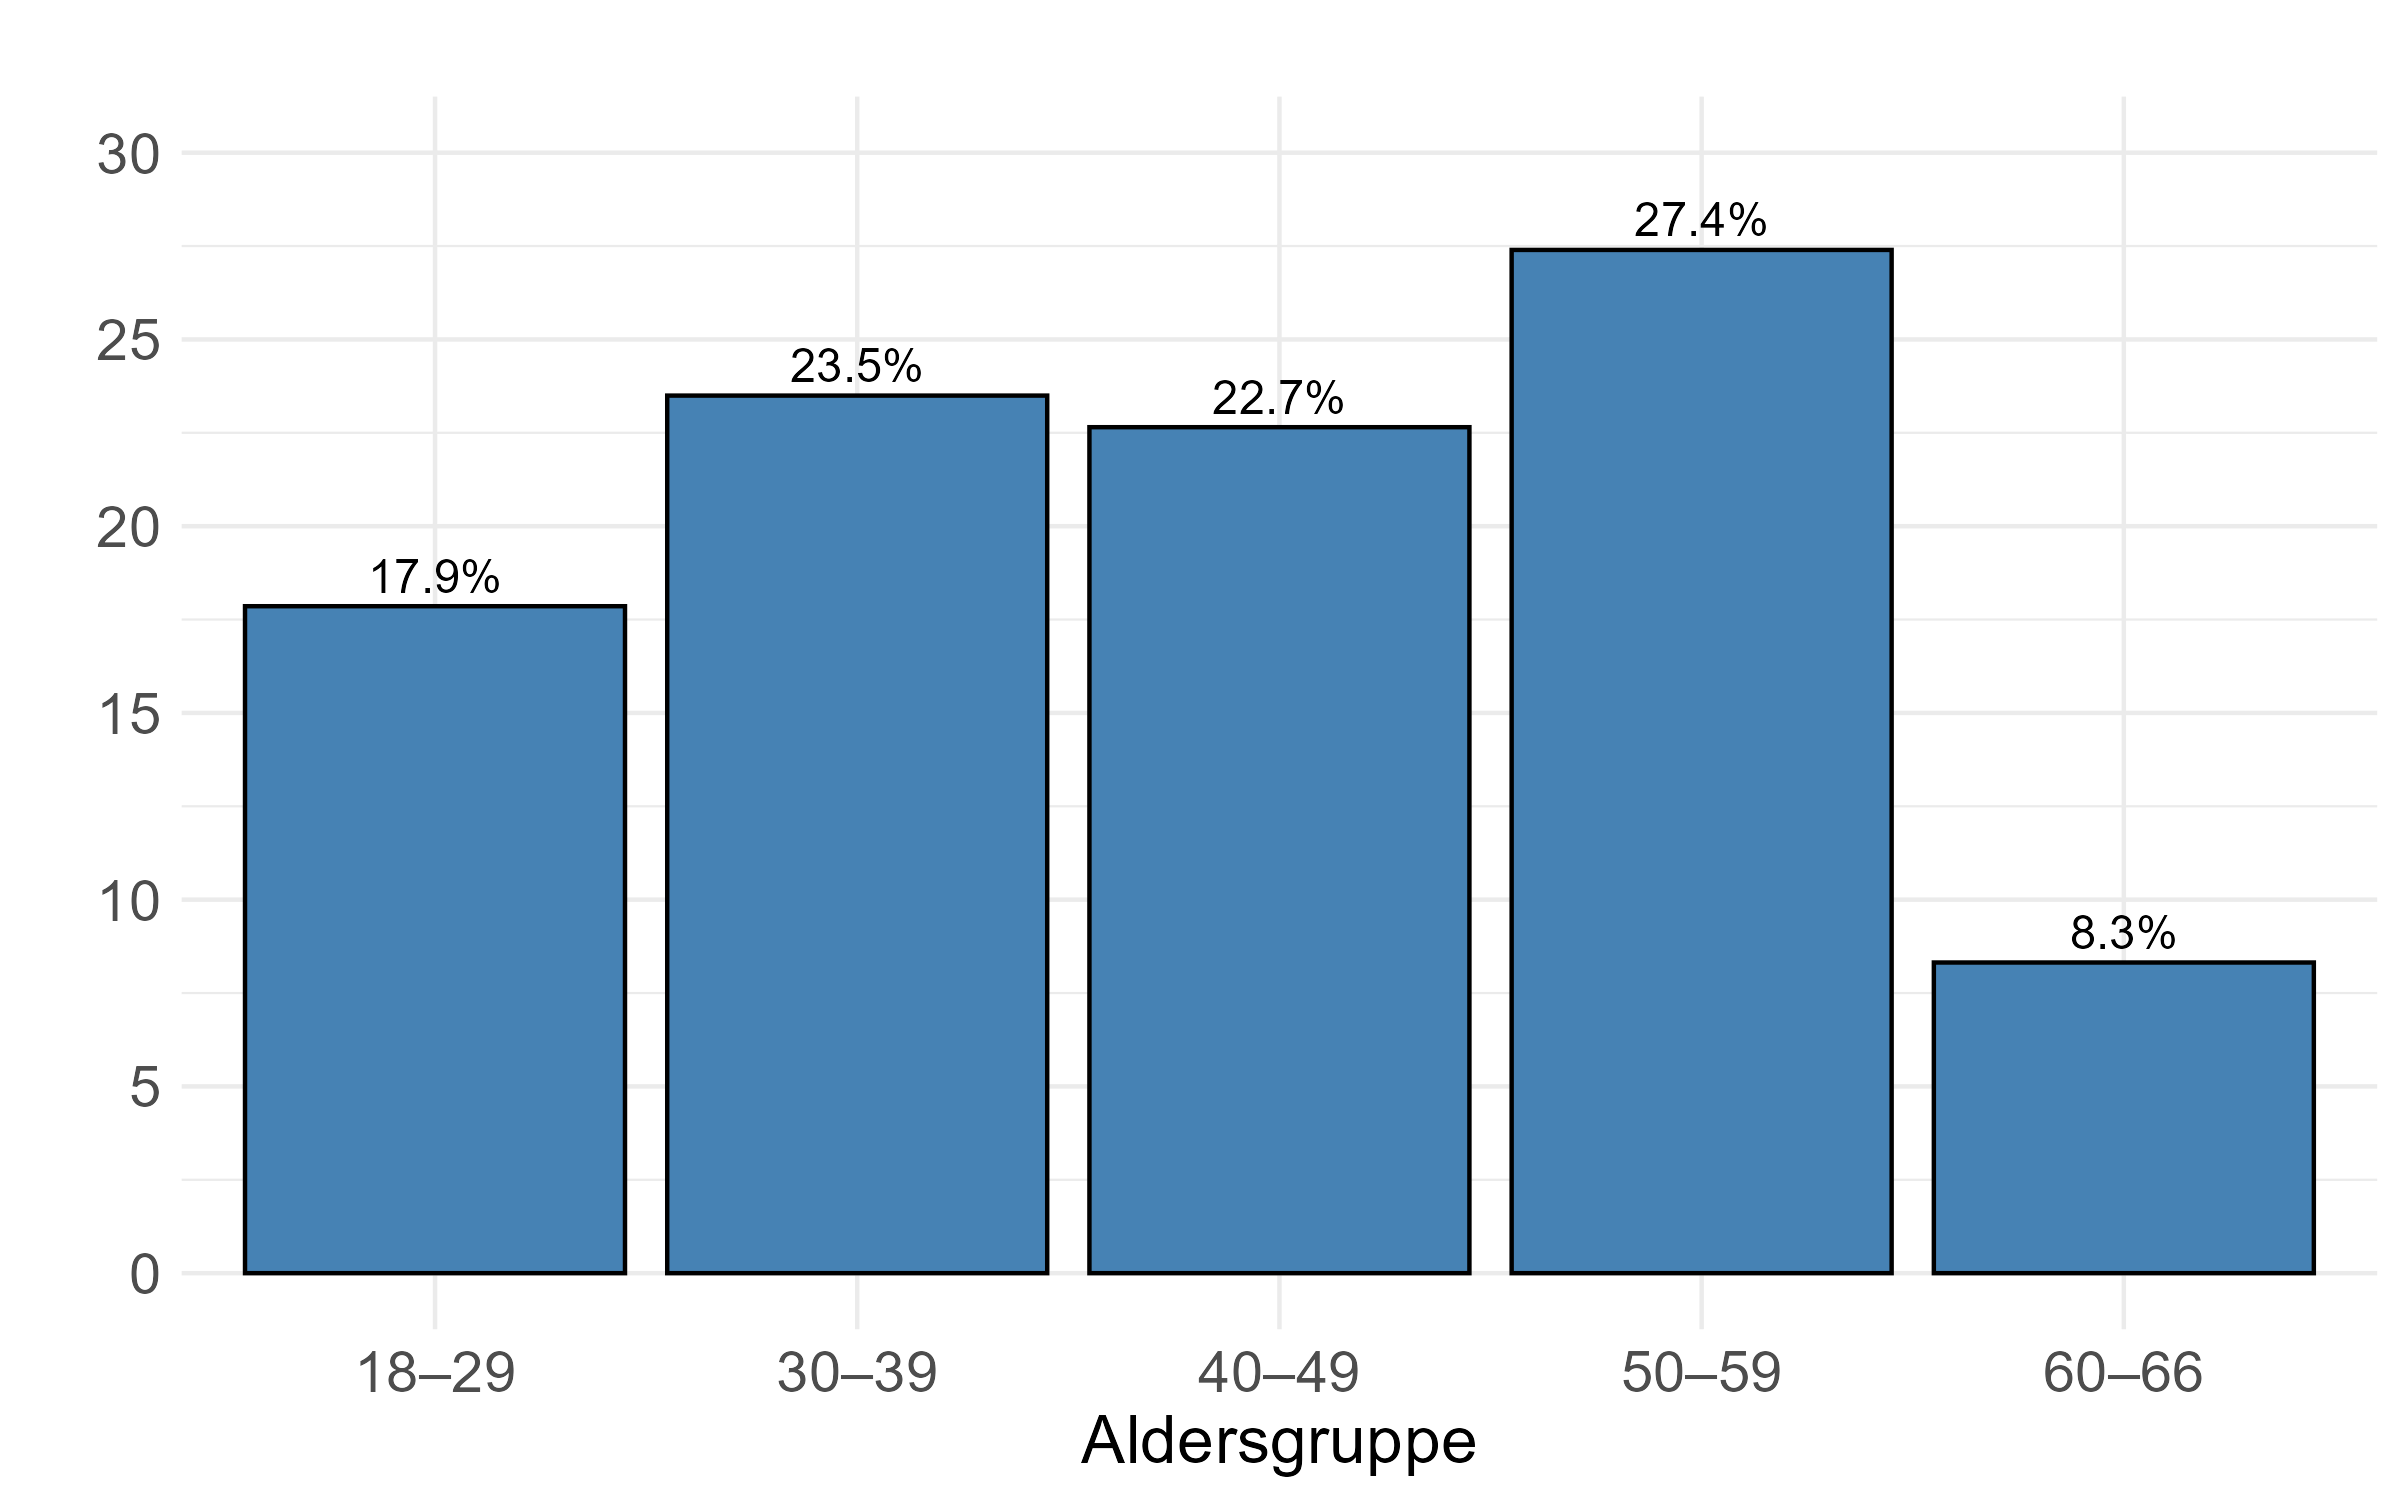
\includegraphics[width=0.8\textwidth]{dokumentobjekter/figurer/fig_3.png}
\end{figure}

I \autoref{fig:histogram_formue} presenteres histogram og tetthetskurve
for bruttofinanskapitalen log-transformert \((1 + x)\) \footnote{Log
  \((1 + x)\) er en vanlig transformasjon for å håndtere høyreskjevhet i
  data, og det kan bidra til å stabilisere variansen og gjøre dataene
  mer normale. Logaritmen gjør at de store verdiene blir mindre og de
  små verdiene blir større.}. Originalt er formuefordelingen høyreskjev,
med en høyere andel av respondentene som har lav formue enn de som har
høy formue noe som kan svekke analysen. Derfor må vi log-transformere
formuefordelingen for å få en mer normalfordelt fordeling både for menn
og kvinner. Når man log-transformerer \((1 + x)\) så tar vi logaritmen
av formueverdiene og legger til 1 for å unngå problemer med nullverdier.

\begin{figure}[H]
\caption{Fordeling av log-transformert bruttofinanskapital}
\label{fig:histogram_formue}
\centering
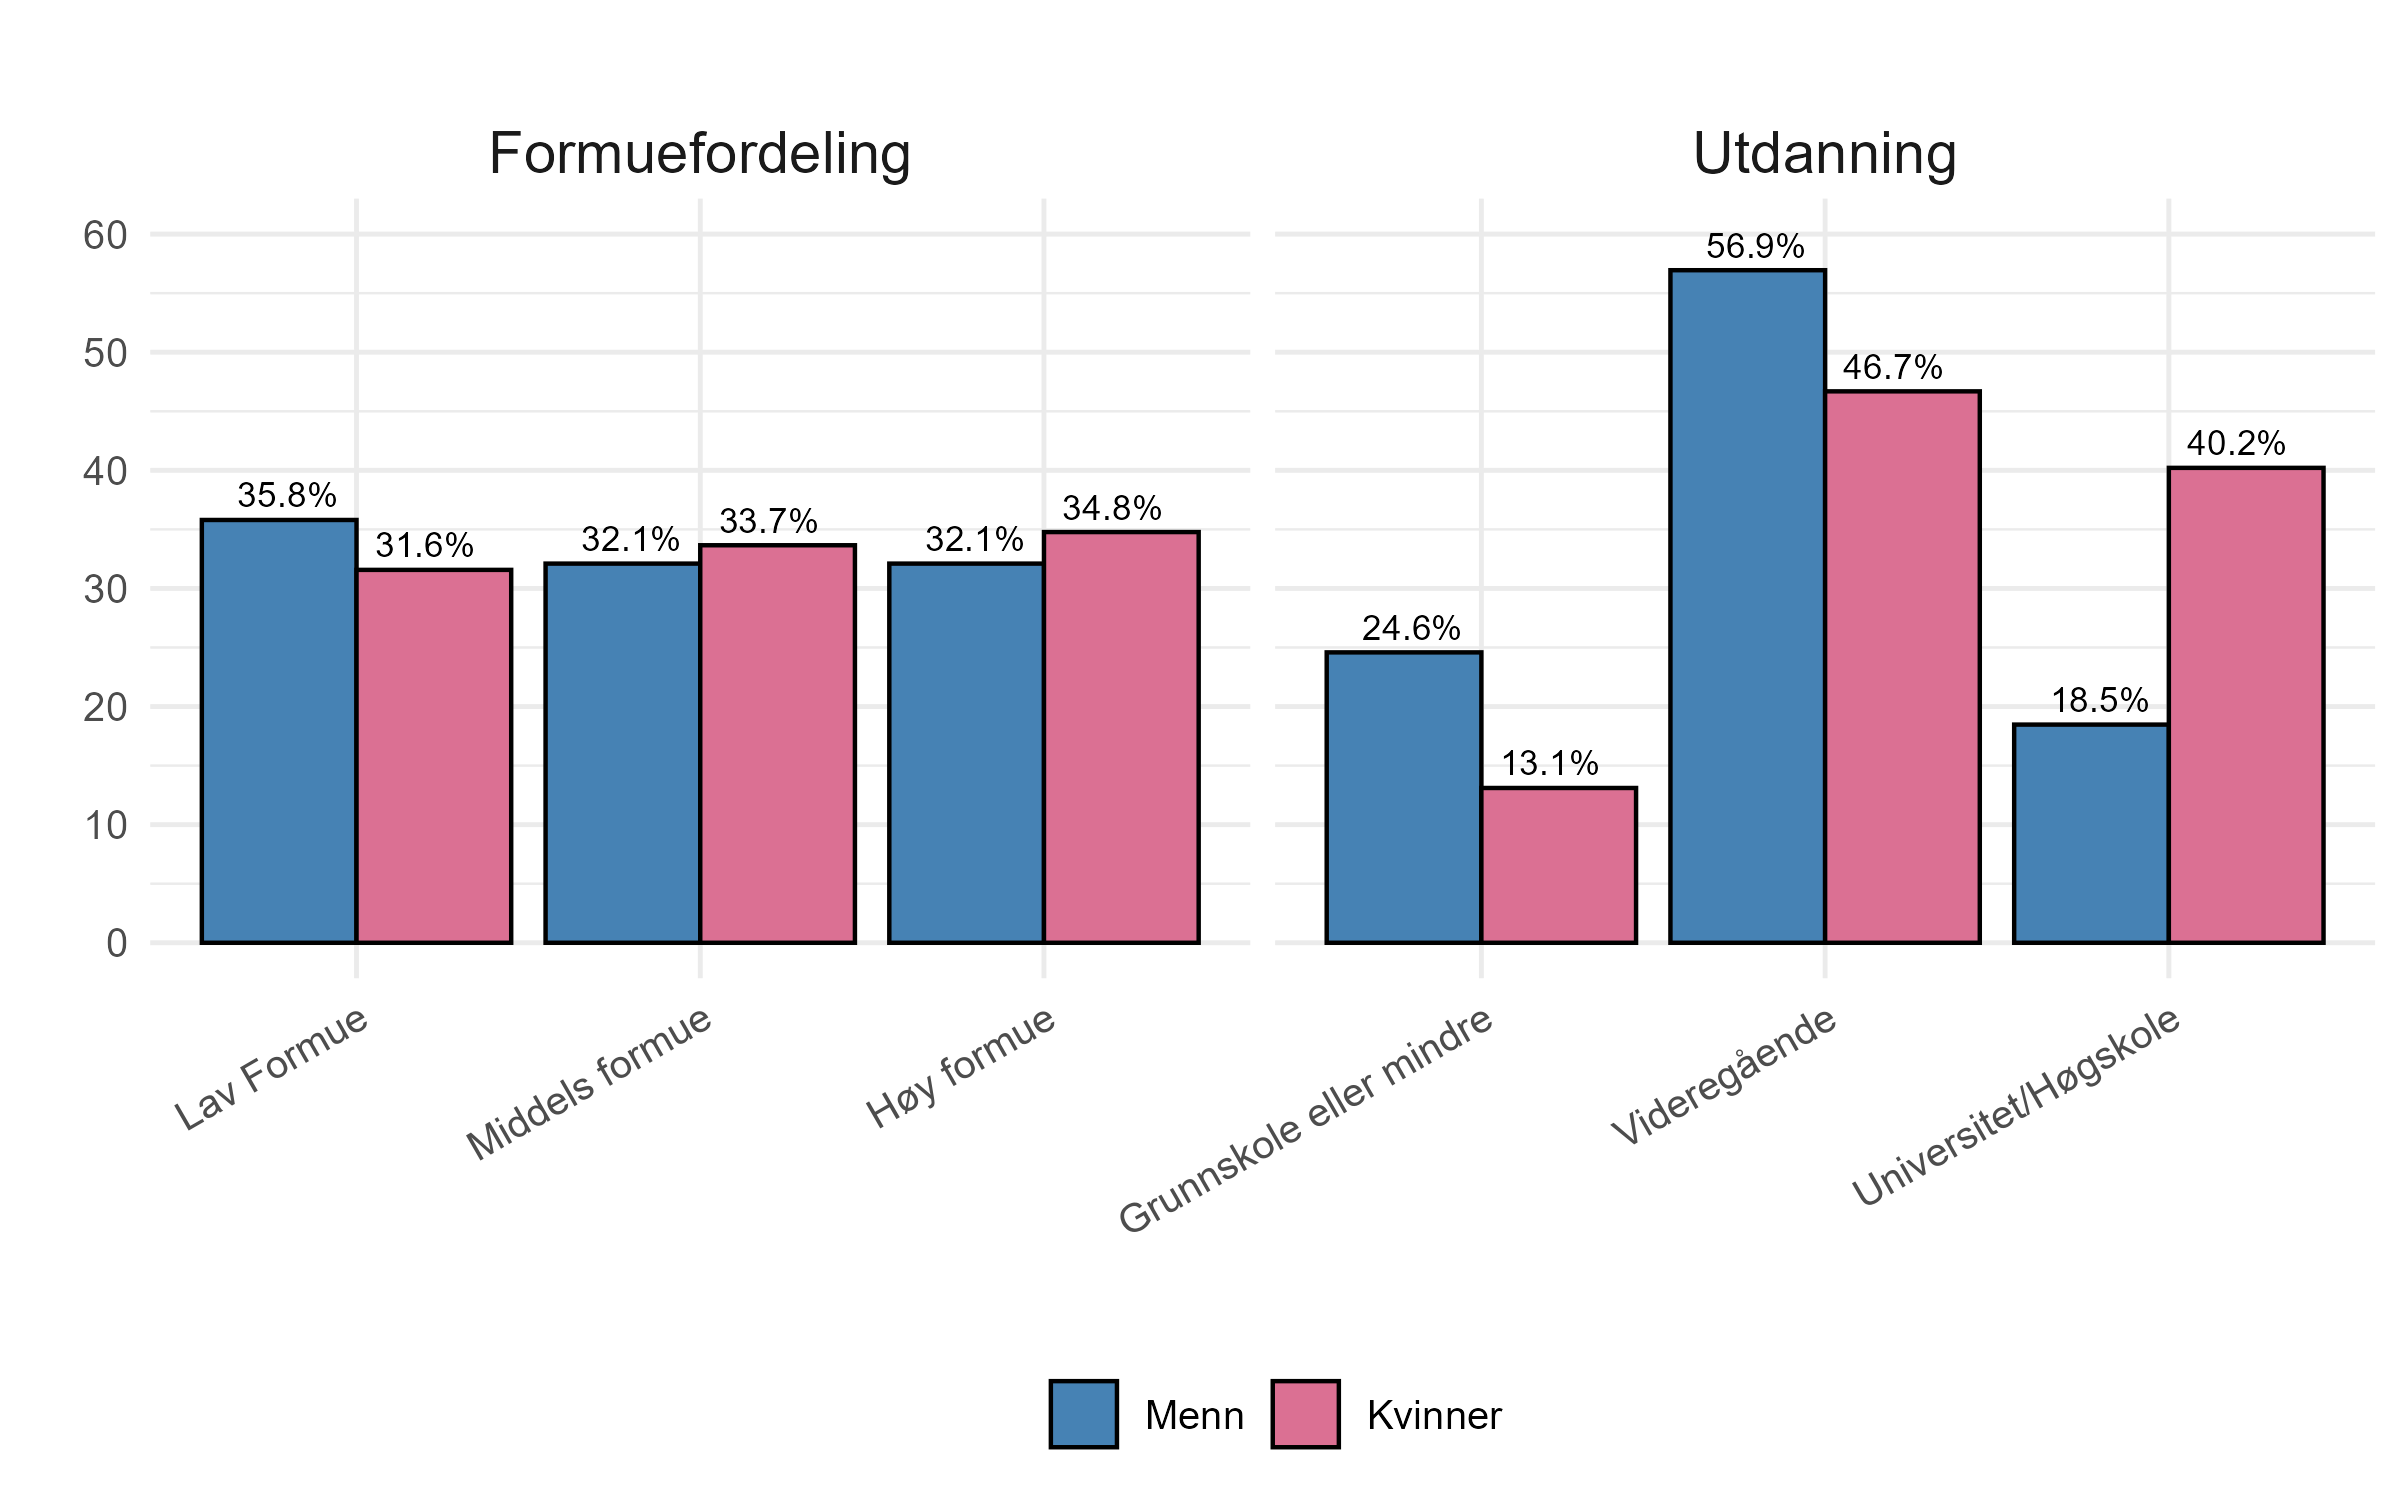
\includegraphics[width=0.8\textwidth]{dokumentobjekter/figurer/fig_4.png}
\end{figure}

Når vi ser på fordelingen av formue- og utdanningsgrupper fordelt på
kjønn i \autoref{fig:barplot_2} så ser vi at det er flest kvinner i
utdanningsgruppen videregående skole med 46.7 prosent, og det samme
gjelder for menn med 56.9 prosent. Mer kvinner enn menn har
universitetsutdannings eller høyere med 40.2 prosent mot kun 18.5
prosent for menn. Menn har også lavest utdanningsnivå med 24.6 prosent i
utdanningsgruppen grunnskole eller mindre, mens kvinner har 13.1 prosent
i den samme utdanningsgruppen. Dette viser oss at menn har lavere
utdanningsnivå enn kvinner, og at kvinner er mer tilbøyelige til å ta
høyere utdanning enn menn.

Formuefordelingen er delt inn i tertiler, som gjør slik at fordelingen
blir jevnt blant de forskjellige formuegruppene både for menn og
kvinner.

\begin{figure}[H]
\caption{Fordeling av formue- og utdanningsgrupper fordelt på kjønn}
\label{fig:barplot_2}
\centering
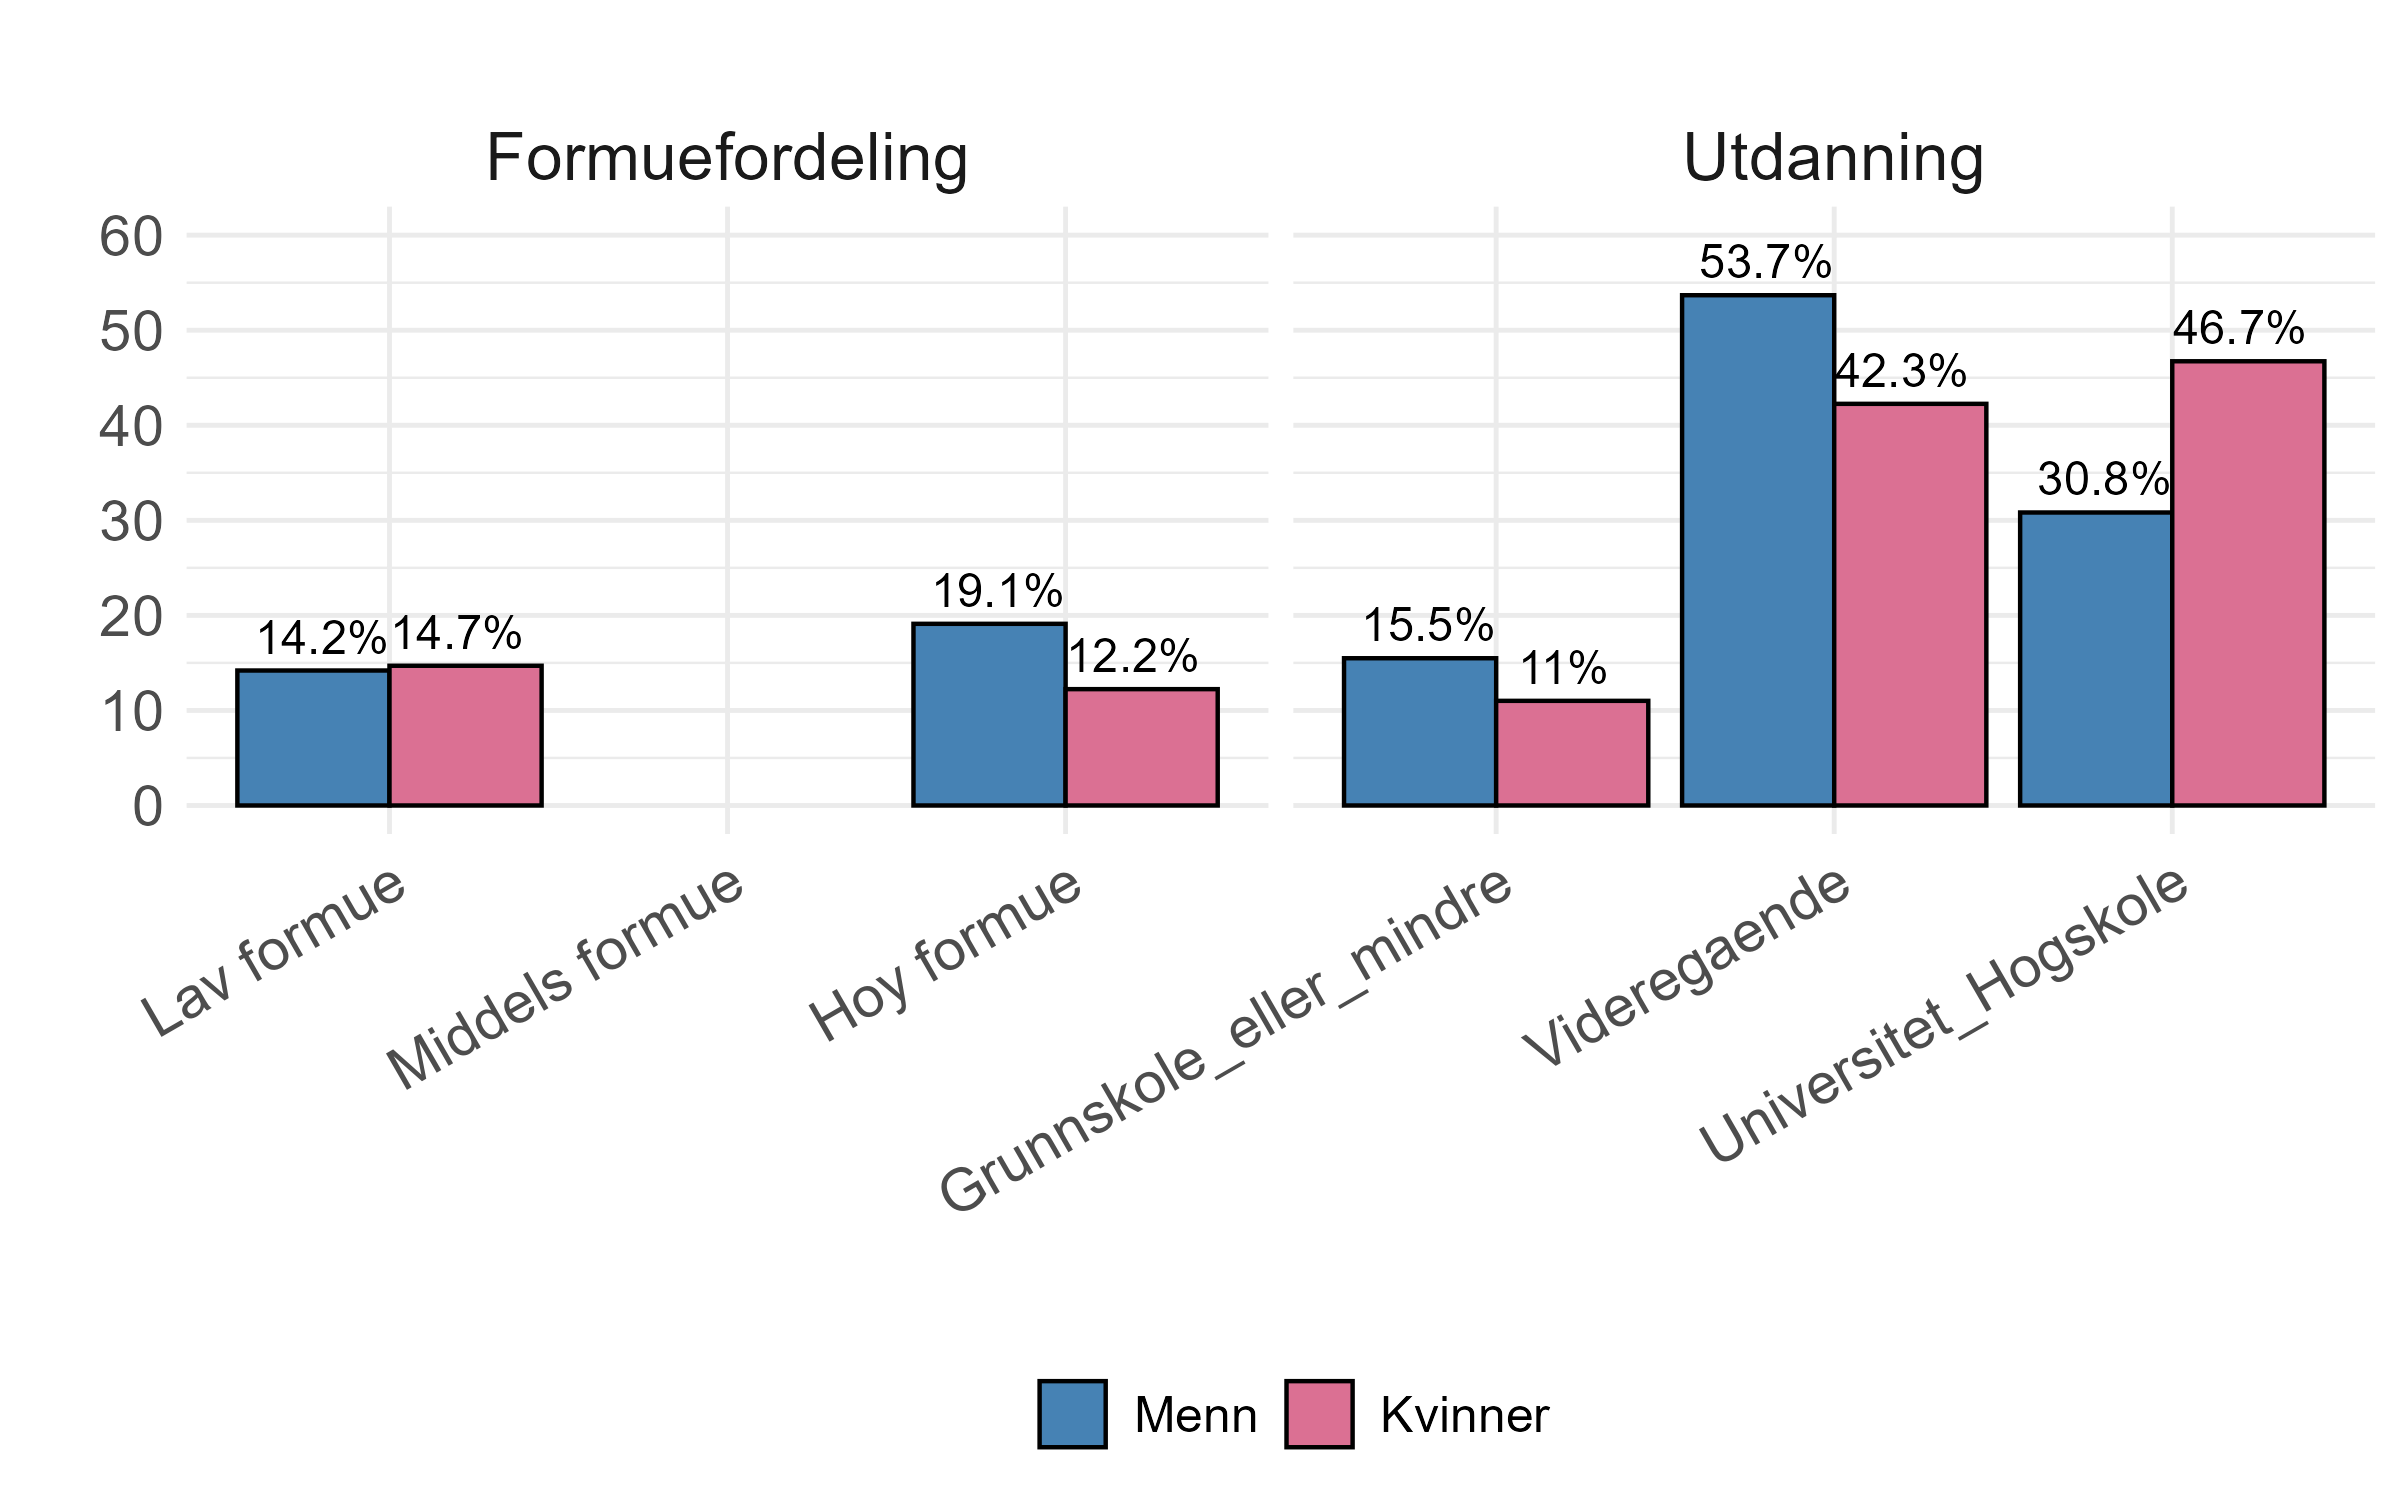
\includegraphics[width=0.8\textwidth]{dokumentobjekter/figurer/fig_5.png}
\end{figure}

I \autoref{fig:boxplot} presenteres et boksplott av sykefravær etter
formuegruppe. Vi kan se at det ikke er store forskjeller i sykefraværet
mellom formuegruppene. Medianen vises i den sorte streken i midten av
boksen, og den viser at sykefraværet med små marginer går ned fra lav
formue, til middels formue og til høy formue. Bunnen og toppen til
boksene viser oss henholdsvis første og tredje kvartil, og de stiplede
linjene viser oss minimum og maksimum sykefravær. Det er også noen
uteliggere som er vist med små prikker, og de viser at det er noen
respondenter som har rapportert sykefravær på over 40 prosent. Dette kan
være at de har vært sykemeldt i en lengre periode. I bakgrunnen av
figuren man man se alle observasjonene spredt utover for en bedre
oversikt siden det er mange observasjoner som går over hverandre i
boksen. Dette er gjort med en funksjon som sprer ut observasjonene litt
for å få en bedre oversikt over dem.

\begin{figure}[H]
\caption{Boksplott av sykefravær etter formuegruppe}
\label{fig:boxplot}
\centering
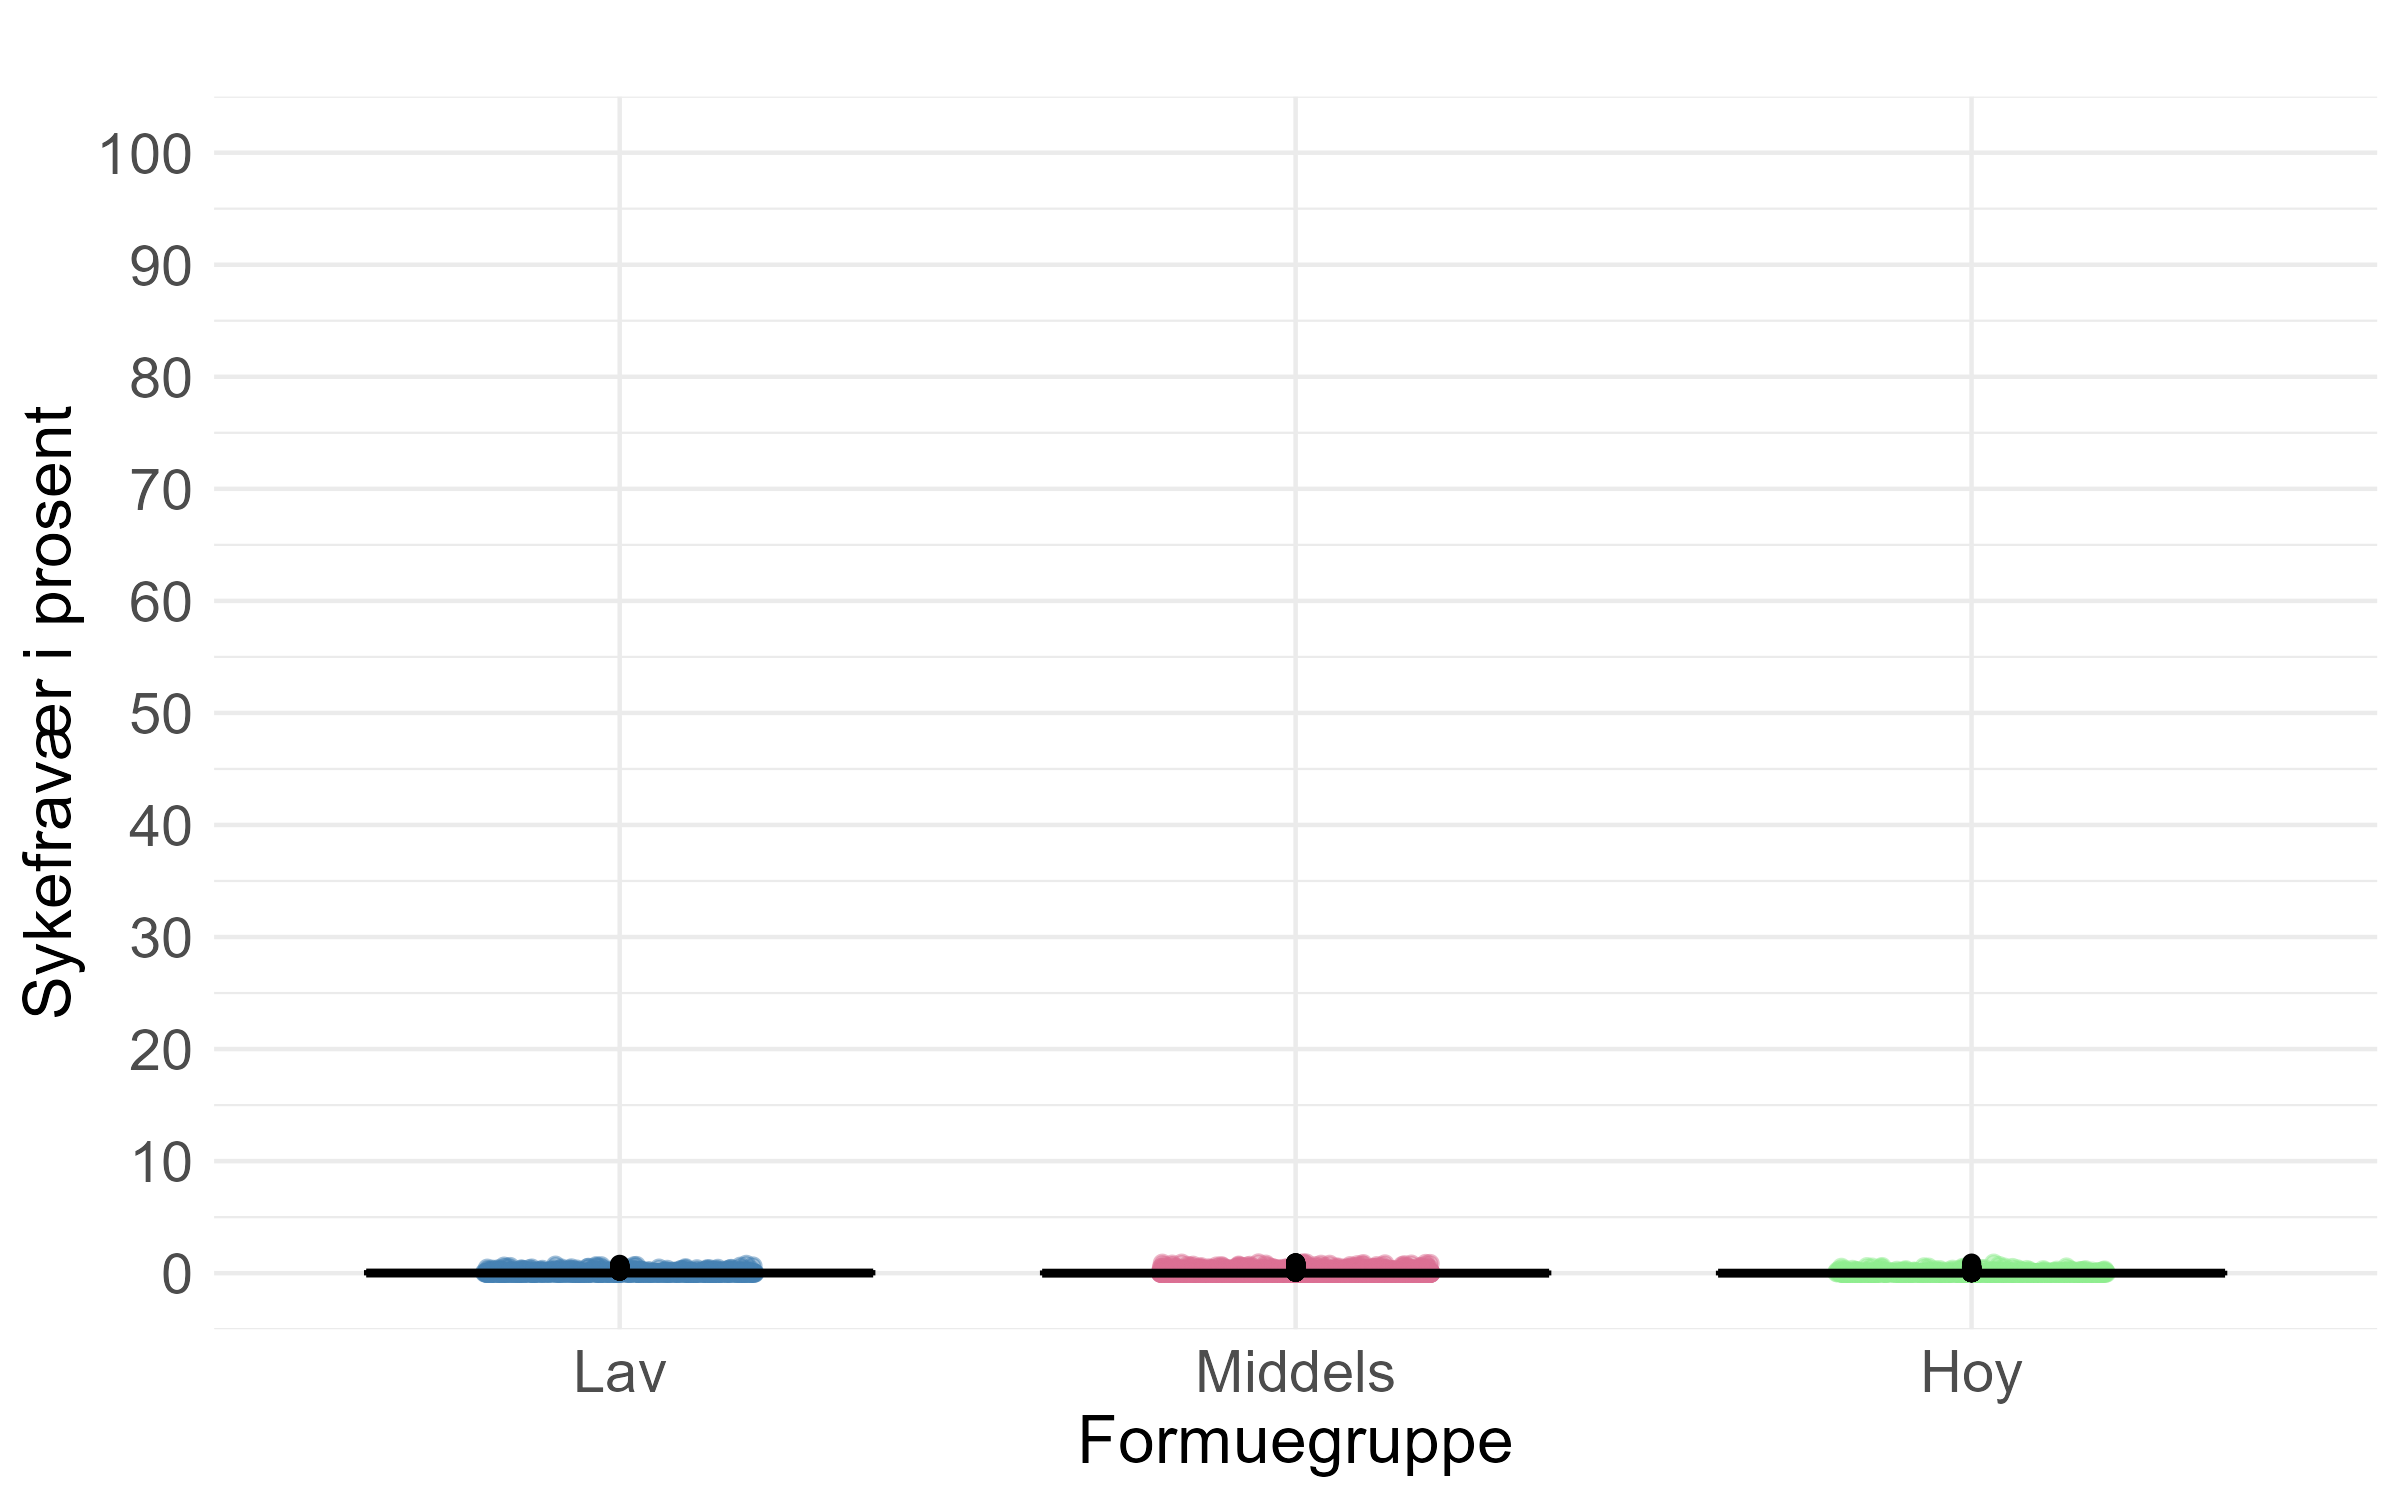
\includegraphics[width=0.8\textwidth]{dokumentobjekter/figurer/fig_6.png}
\end{figure}

I \autoref{fig:boxplot_2} presenteres et boksplott av sykefravær etter
utdanningsnivå. Vi ser at sykefraværet er veldig jevnt mellom
utdanningsnivåene. Medianen er litt over 10 prosent, og som tidligere
vet vi at gjennomsnittlig sykefravær er lavere for høyt utdannede og
litt lavere for de med lavere utdanning.

\begin{figure}[H]
\caption{Boksplott av sykefravær etter utdanningsnivå}
\label{fig:boxplot_2}
\centering
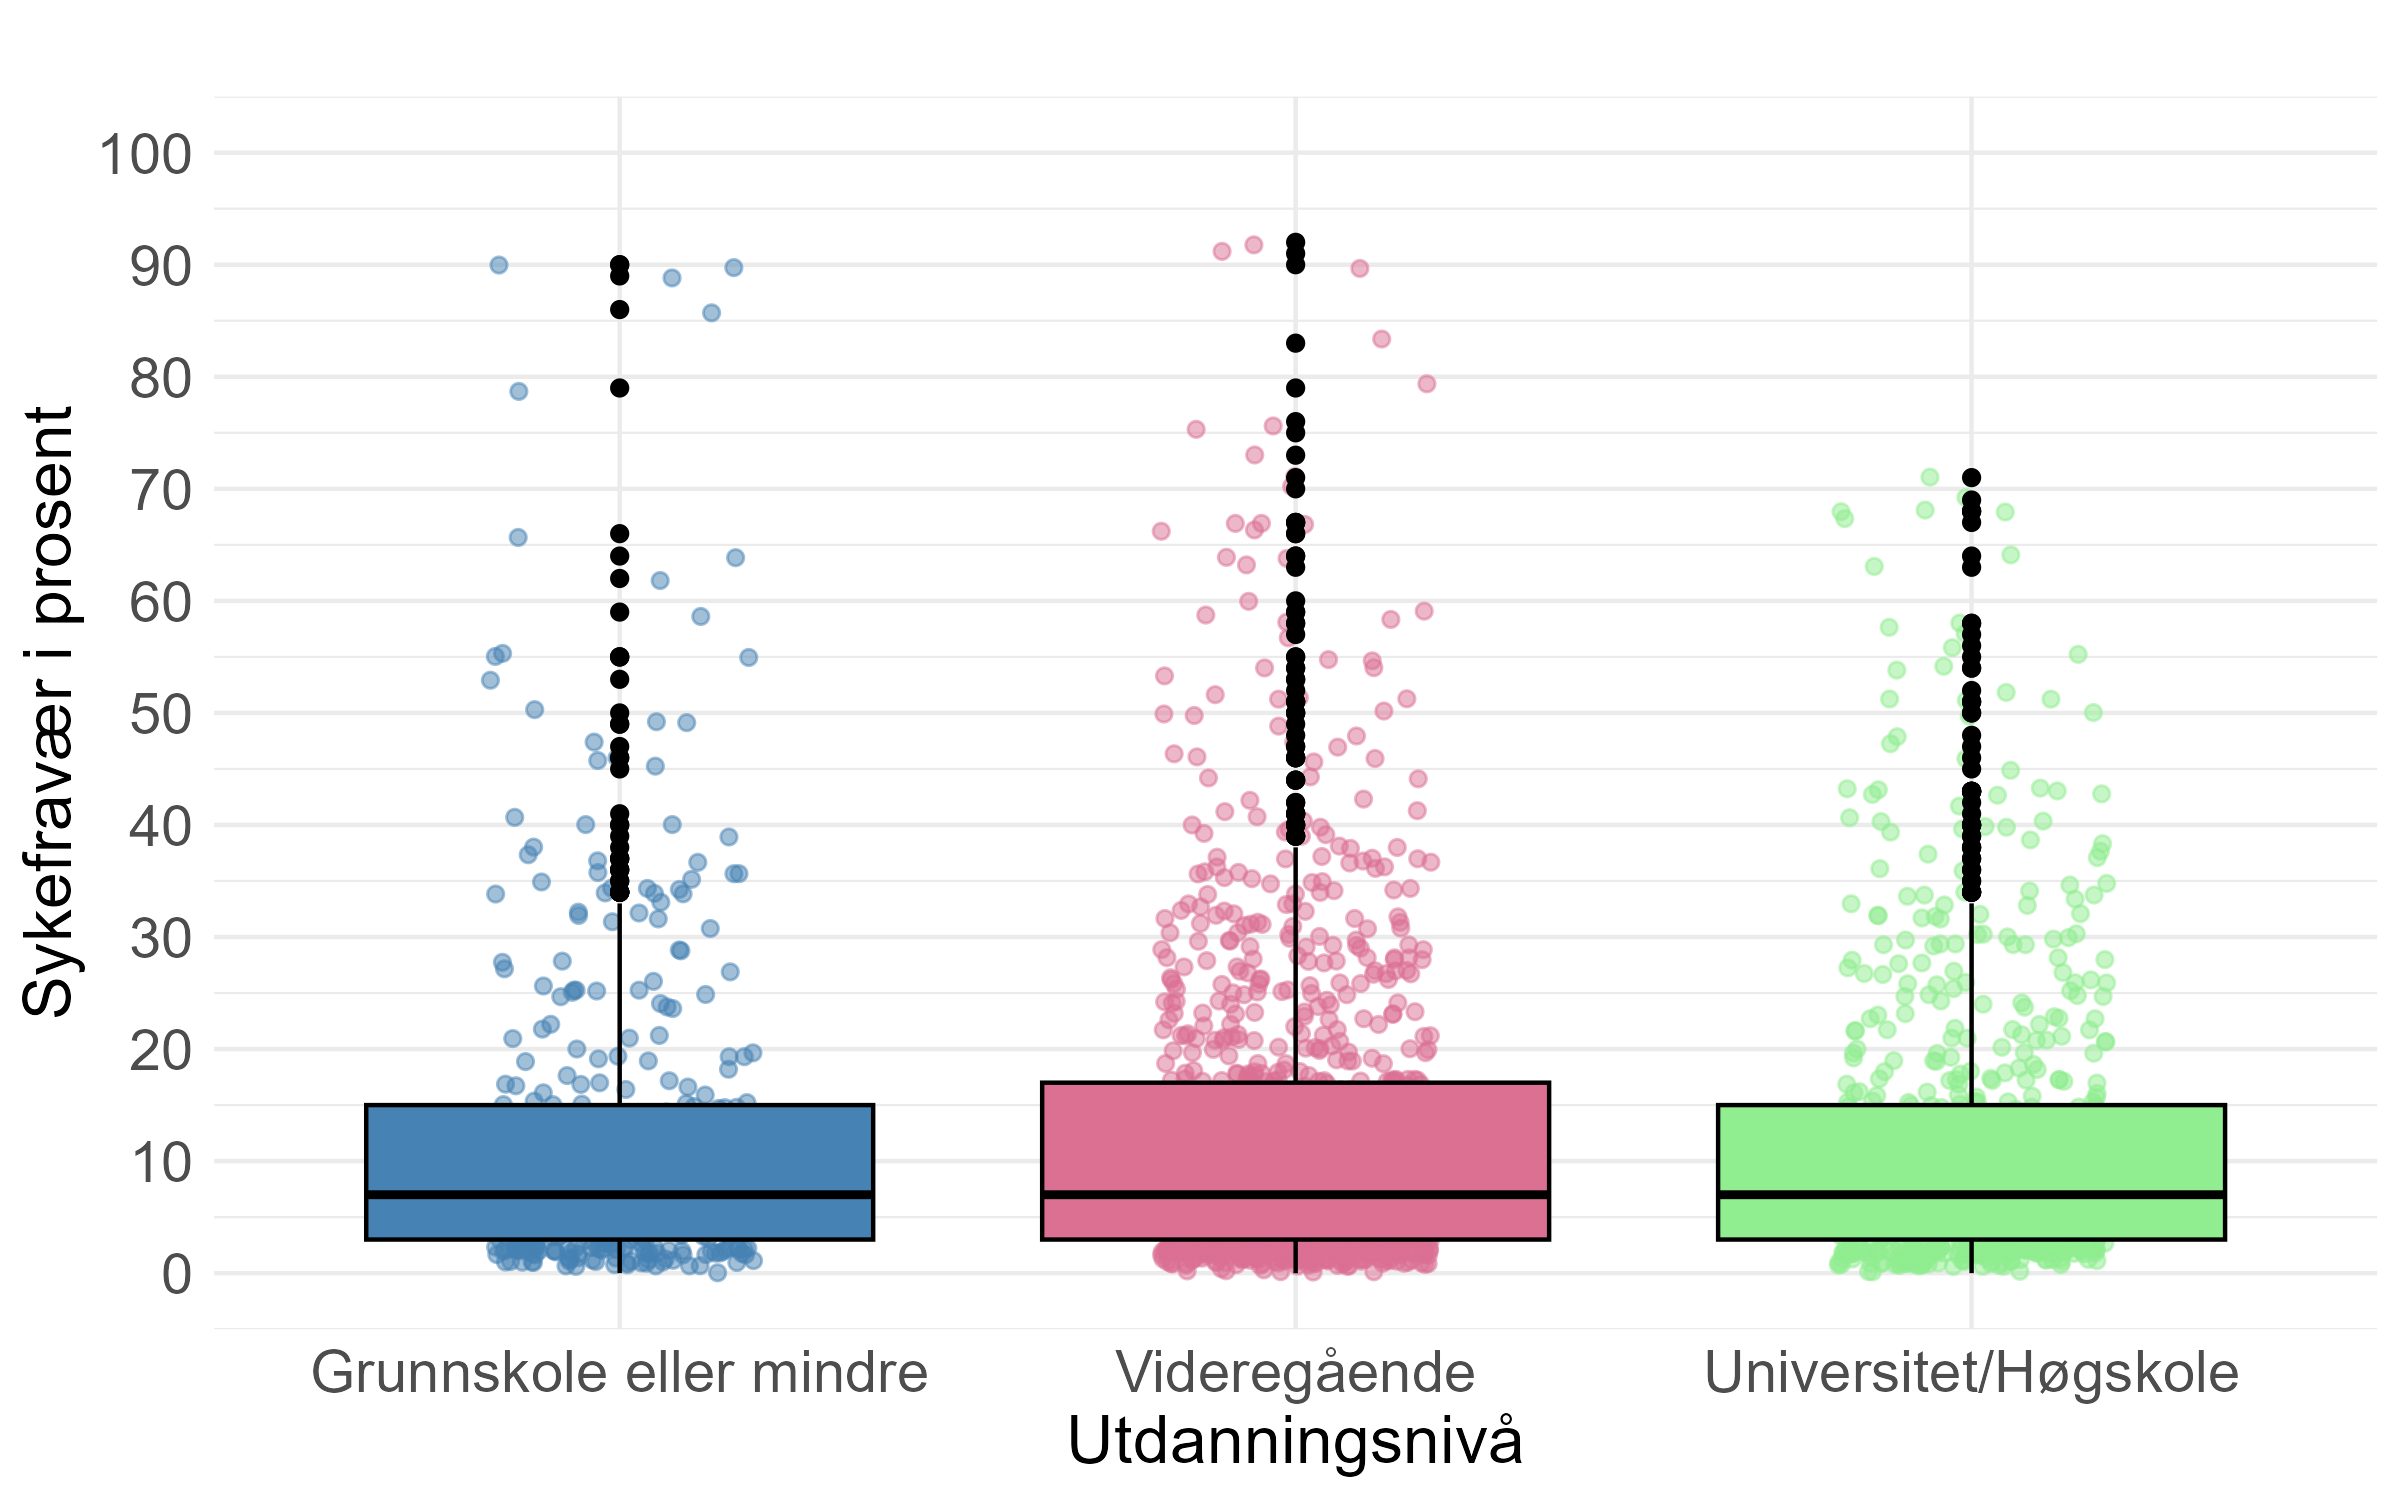
\includegraphics[width=0.8\textwidth]{dokumentobjekter/figurer/fig_7.png}
\end{figure}

Korrelationheatmap om vi får tid her til latente variabler.

\subsection{Metode}\label{metode}

I oppgaven vil vi bruke en kvantitativ metode for å analysere
sammenhengen mellom formue og sykefravær. Vi vil bruke en Structural
Equation Model (SEM) for å teste hypotesene våre, og vi vil kontrollere
for andre relevante faktorer som kan påvirke sykefraværet. SEM er en
statistisk metode som gjør det mulig å teste komplekse modeller med
flere variabler, og som kan håndtere både direkte og indirekte
sammenhenger mellom variablene. Vi vil bruke R for å gjennomføre
analysen, og vi vil bruke pakker som x og x for å implementere
SEM-modellen.

\subsection{Structural Equation Model
(SEM)}\label{structural-equation-model-sem}

Formue inngår i modellen på tre måter: som en direkte
forklaringsvariabel for sykefravær, som en indirekte påvirkning via
motivasjon, og som en modererende variabel som endrer effekten av
jobbkrav og jobbressurser.

Vi antar at formue fungerer som et mål på økonomisk trygghet og
handlingsrom. Personer med høyere formue har trolig mer fleksibilitet
til å håndtere belastninger på jobb, og vil kunne tåle høye jobbkrav
uten samme negative effekt på helse og fravær. Samtidig antar vi at
høyere formue gir høyere jobbmotivasjon fordi økonomisk trygghet gjør
det lettere å finne mening, utvikling og balanse i arbeidet.

På bakgrunn av dette har vi inkludert interaksjonsledd mellom formue og
jobbkrav (\(JD_i FN_i\)), samt mellom formue og jobbressurser
(\(JR_i FN_i\)), for å fange opp slike modererende effekter. Vi har også
modellert motivasjon som en medierende variabel, hvor formue kan påvirke
motivasjonen, som igjen kan påvirke sykefravær.

Dette modellvalget bygger videre på JD-R-rammeverket, men inkluderer
økonomisk kontekst som en faktor som kan endre hvordan individer
påvirkes av jobbsituasjonen. Ved å bruke en SEM-modell kan vi teste både
de direkte og indirekte sammenhengene mellom formue og sykefravær.

\subsubsection{Ligning til modellen}\label{ligning-til-modellen}

\[
SF_i = \beta_0 + \beta_1 JK_i + \beta_2 JR_i + \beta_3 FN_i + \beta_4 (JD_iFN_i) + \beta_5 (JR_i FN_i) + \beta_6 M_i + \Sigma_j \gamma_{j}X_{ij} + \epsilon_{1i}
\]

\[
M_i = \alpha_0 + \alpha_1 JR_i + \alpha_2 FN_i + \Sigma_k \alpha_{3k}X_{ik} + \epsilon_{2i} \tag{Motivasjon}\label{eq:motivasjon}
\]

\subsubsection{Forklaring av alle deler i
modellen}\label{forklaring-av-alle-deler-i-modellen}

\begin{table}[H]
\centering
\begin{tabular}{lr}
\toprule
Symbol & Forklaring \\ 
\midrule
$SF_i$ & Prosentandel av avtalte arbeidsdager arbeidstaker i er fraværende (sykefravær) \\
$JD_i$ & Latent jobbkrav score (høyere = mer krav) \\
$JR_i$ & Latent jobbressurser score (høyere = mer støtte/autonomi) \\
$FN_i$ & Logaritmen eller prosentil rangeringen av individets (eller husholdningens) formue \\
$M_i$ & Motivasjons-/engasjements score \\
$X_{ij}$ & Kontrollvariabler (alder, kjønn, utdanning …), alle gjennomsnittssentrert \\
$\epsilon_{1i}, \epsilon_{2i}$ & Forstyrrelser (null-gjennomsnitt, ukorrelerte med prediktorer) \\  
$\alpha_{3j} $ & Koeffisienter for kontrollvariablene på Motivasjon i motivasjonsmodellen \\
$\gamma_{j} $ & Koeffisienter for kontrollvariablene i på sykefravær i sykefraværmodellen \\
\hline
\end{tabular}
\caption{Oversikt over variabler i modellen}
\label{tab:variabler}
\end{table}

\subsubsection{Beskrivning av metode}\label{beskrivning-av-metode}

Vår medierende variabel Motivasjon (\(M_i\)) i \autoref{eq:motivasjon}
er modellert som en funksjon av jobbressurser (\(JR_i\)) og formue
(\(FN_i\)), samt kontrollvariabler. Her forventer vi at \(\alpha_1 > 0\)
i tråd med JD-R modellen og Langseth-Eide \& Vittersø (2021) hvor
jobbressurser bygger engasjement og motivasjon. Vi forventer også at
\(\alpha_2 > 0\) som betyr at høyere formue vil føre til høyere
motivasjon. Dette bygger på antagelsen om at økonomisk trygghet
reduserer stress og frigjør mental kapasitet. Det bygger også på at på
at utsikter til økonomisk fremgang, eller fraværet av en følelse av at
det ikke er mulig å bli økonomisk trygg som kan oppstå ved stor ulikhet
Gesiarz et al. (2020), og at du dermed kan styrke den indre motivasjonen
for arbeidet.

\subsubsection{Hypoteser}\label{sec-hypot}

Ut fra vår hovedmodell for sykefravær:

\[
SF_i = \beta_0 + \beta_1 JK_i + \beta_2 JR_i + \beta_3 FN_i + \beta_4 (JD_i FN_i) + \beta_5 (JR_i FN_i) + \beta_6 M_i + \Sigma_j \gamma_{j}X_{ij} + \epsilon_{1i}
\] formulerer vi følgende hypoteser:

\paragraph{\texorpdfstring{Hypotese 1(H1): \(\beta_1 > 0\) Høyere
jobbkrav gir høyere
sykefravær}{Hypotese 1(H1): \textbackslash beta\_1 \textgreater{} 0 Høyere jobbkrav gir høyere sykefravær}}\label{hypotese-1h1-beta_1-0-huxf8yere-jobbkrav-gir-huxf8yere-sykefravuxe6r}

Dette er en grunnleggende antagelse i JD-R-modellen (Schaufeli \&
Bakker, 2004; Vander Elst et al., 2016). Høye krav (fysiske, psykiske,
emosjonelle) tærer på individets ressurser og kan føre til utbrenthet og
helseplager, som igjen øker sannsynligheten for sykefravær.

\paragraph{\texorpdfstring{Hypotese 2(H2): \(\beta_2 < 0\) Høyere
jobbressurser gir lavere
sykefravær}{Hypotese 2(H2): \textbackslash beta\_2 \textless{} 0 Høyere jobbressurser gir lavere sykefravær}}\label{hypotese-2h2-beta_2-0-huxf8yere-jobbressurser-gir-lavere-sykefravuxe6r}

Jobbressurser (støtte, autonomi, tilbakemelding) fungerer som
beskyttende faktorer. De hjelper ansatte med å håndtere krav, oppnå mål
og fremmer personlig vekst, noe som fører til høyere engasjement og
bedre helse, og dermed lavere fravær (Langseth-Eide \& Vittersø, 2021).

\paragraph{\texorpdfstring{Hypotese 3(H3): \(\beta_3 < 0\) Høyere
formuenivå gir lavere
sykefravær}{Hypotese 3(H3): \textbackslash beta\_3 \textless{} 0 Høyere formuenivå gir lavere sykefravær}}\label{hypotese-3h3-beta_3-0-huxf8yere-formuenivuxe5-gir-lavere-sykefravuxe6r}

Vi forventer en direkte, gunstig effekt av formue på sykefravær. Formue
fungerer som en ``buffer'' mot levekårsproblemer (Hattrem, n.d.;
Normann, 2009) og gir økonomisk trygghet. Dette kan redusere generelt
stressnivå og forbedre helsen, slik funn fra Jaeggi et al. (2021)
indikerer (høyere formue -\textgreater{} lavere blodtrykk, færre
luftveissykdommer). Økonomisk trygghet kan også gi bedre tilgang til
helsetjenester og en større evne til å håndtere helseutfordringer uten å
måtte ty til langvarig fravær.

\paragraph{\texorpdfstring{Hypotese 4(H4): \(\beta_4 < 0\) Høyere
formuenivå demper de negative effektene til høyere
jobbkrav}{Hypotese 4(H4): \textbackslash beta\_4 \textless{} 0 Høyere formuenivå demper de negative effektene til høyere jobbkrav}}\label{hypotese-4h4-beta_4-0-huxf8yere-formuenivuxe5-demper-de-negative-effektene-til-huxf8yere-jobbkrav}

Dette er en modereringshypotese. Vi tror at formue reduserer
sensitiviteten for jobbkrav. For en person med lav formue kan høye krav
oppleves som svært truende, da konsekvensene av å ikke mestre (for eks,
miste jobben) er store. For en person med høy formue, gir den økonomiske
tryggheten en mental ``pute'' som gjør at de samme kravene ikke utløser
like mye stress. Dette er i tråd med Üngüren et al. (2021), som fant at
økonomisk velvære fungerte som en slik buffer. Den marginale effekten av
jobbkrav er
\(\frac{\partial SF_i}{\partial JD_i} = \beta_1 + \beta_4 FN_i\). En
negativ \(\beta_4\) betyr at effekten av JK på SF blir mindre etter
hvert som FN øker.

\paragraph{\texorpdfstring{Hypotese 5(H5): \(\beta_5 > 0\) Høyere
formuenivå demper den reduserende effekten av høyere jobbressurser på
sykefravær}{Hypotese 5(H5): \textbackslash beta\_5 \textgreater{} 0 Høyere formuenivå demper den reduserende effekten av høyere jobbressurser på sykefravær}}\label{hypotese-5h5-beta_5-0-huxf8yere-formuenivuxe5-demper-den-reduserende-effekten-av-huxf8yere-jobbressurser-puxe5-sykefravuxe6r}

Dette er vår andre modereringshypotese, basert på en antagelse om
avtagende grensenytte. Vi antar at jobbressurser har størst relativ
effekt for de med lav formue. For en person med lav formue og potensielt
høy økonomisk usikkerhet, vil en økning i jobbressurser som er en
negativ effekt på sykefravær ha en stor reduserende effekt på
sykefravær. En person med høy formue, som allerede har høy økonomisk
trygghet, vil den samme økningen i jobbressurser ha en mindre
tilleggseffekt. Effekten er altså sterkest for de med lav formue, og
blir svakere jo høyere formuen blir. Den marginale effekten av
jobbressurser er
\(\frac{\partial SF_i}{\partial JR_i} = \beta_2 + \beta_5 FN_i\). Siden
\(\beta_2 < 0\) er negativ, vil en positiv \(\beta_5\) gjøre den totale
effekten mindre negativ etter hvert som \(FN_i\) øker.

\paragraph{\texorpdfstring{Hypotese 6(H6): Indirekte effekt via
motivasjon
\(\alpha_2\beta_6 < 0\)}{Hypotese 6(H6): Indirekte effekt via motivasjon \textbackslash alpha\_2\textbackslash beta\_6 \textless{} 0}}\label{hypotese-6h6-indirekte-effekt-via-motivasjon-alpha_2beta_6-0}

Vi forventer en indirekte vei der formue påvirker sykefravær gjennom
motivasjon. Som nevnt AUTOREF, forventer vi at høyere formue øker
motivasjonen \(\alpha_2 > 0\) som ved å redusere finansiell usikkerhet,
og gode fremtidsutsikter. Videre forventer vi at høyere
motivasjon/engasjement reduserer sykefraværet (\(\beta_6 <0\)), slik
Langseth-Eide \& Vittersø (2021) fant. Samlet sett gir dette en
forventning om en negativ indirekte effekt \(\alpha_2 \beta_6 <0\), som
betyr at en del av formues positive effekt på helse/nærvær går via økt
arbeidsglede og engasjement som igjen gir lavere sykefravær.

\newpage

\section{Analyse}\label{analyse}

\#wtf ai hjelp for nu.

\begin{verbatim}
lavaan 0.6-19 ended normally after 178 iterations

  Estimator                                         ML
  Optimization method                           NLMINB
  Number of model parameters                        70

  Number of observations                          2128

Model Test User Model:
                                              Standard      Scaled
  Test Statistic                              4730.631    2059.218
  Degrees of freedom                               374         374
  P-value (Chi-square)                           0.000       0.000
  Scaling correction factor                                  2.297
    Yuan-Bentler correction (Mplus variant)                       

Model Test Baseline Model:

  Test statistic                             12929.500    4705.697
  Degrees of freedom                               420         420
  P-value                                        0.000       0.000
  Scaling correction factor                                  2.748

User Model versus Baseline Model:

  Comparative Fit Index (CFI)                    0.652       0.607
  Tucker-Lewis Index (TLI)                       0.609       0.558
                                                                  
  Robust Comparative Fit Index (CFI)                         0.671
  Robust Tucker-Lewis Index (TLI)                            0.631

Loglikelihood and Information Criteria:

  Loglikelihood user model (H0)             -94632.047  -94632.047
  Scaling correction factor                                  6.994
      for the MLR correction                                      
  Loglikelihood unrestricted model (H1)     -92266.732  -92266.732
  Scaling correction factor                                  3.038
      for the MLR correction                                      
                                                                  
  Akaike (AIC)                              189404.094  189404.094
  Bayesian (BIC)                            189800.499  189800.499
  Sample-size adjusted Bayesian (SABIC)     189578.101  189578.101

Root Mean Square Error of Approximation:

  RMSEA                                          0.074       0.046
  90 Percent confidence interval - lower         0.072       0.045
  90 Percent confidence interval - upper         0.076       0.047
  P-value H_0: RMSEA <= 0.050                    0.000       1.000
  P-value H_0: RMSEA >= 0.080                    0.000       0.000
                                                                  
  Robust RMSEA                                               0.070
  90 Percent confidence interval - lower                     0.067
  90 Percent confidence interval - upper                     0.073
  P-value H_0: Robust RMSEA <= 0.050                         0.000
  P-value H_0: Robust RMSEA >= 0.080                         0.000

Standardized Root Mean Square Residual:

  SRMR                                           0.056       0.056

Parameter Estimates:

  Standard errors                             Sandwich
  Information bread                           Observed
  Observed information based on                Hessian

Latent Variables:
                   Estimate  Std.Err  z-value  P(>|z|)   Std.lv  Std.all
  JK =~                                                                 
    For_mye_arbd_c    1.000                               0.548    0.605
    Hoyt_rbdstmp_c    0.465    0.057    8.096    0.000    0.255    0.365
    Ekstra_arbed_c    1.378    0.156    8.833    0.000    0.755    0.541
  JR =~                                                                 
    Stotte_sjef_c     1.000                               0.760    0.615
    Stotte_kollg_c    0.510    0.034   14.799    0.000    0.388    0.411
    Tlbkmldng_sjf_    1.037    0.046   22.351    0.000    0.789    0.626
    Arbedsrslttr_c    1.240    0.054   22.879    0.000    0.943    0.682
    Grd_slvbstmm__    0.750    0.080    9.358    0.000    0.570    0.517
    Grd_slvbs_____    0.727    0.085    8.584    0.000    0.553    0.522
    Grad_rbdstmp_c    0.694    0.078    8.875    0.000    0.527    0.497
    Grd_pvrk_bsl__    0.808    0.077   10.476    0.000    0.615    0.591
  JKxFN =~                                                              
    Fr_my_rb___LFC    1.000                               0.896    0.486
    Hyt_rbds___LFC    0.658    0.172    3.822    0.000    0.589    0.415
    Ekstr_rb___LFC    1.945    0.582    3.342    0.001    1.743    0.599
  JRxFN =~                                                              
    Sttt_sjf___LFC    1.000                               1.626    0.651
    Sttt_kll___LFC    0.435    0.114    3.803    0.000    0.707    0.358
    Tlbkmld____LFC    0.913    0.241    3.783    0.000    1.485    0.578
    Arbdsrsl___LFC    1.183    0.213    5.552    0.000    1.925    0.660
    Grd_slv____LFC    0.654    0.221    2.961    0.003    1.064    0.457
    Grd________LFC    0.743    0.353    2.108    0.035    1.208    0.564
    Grd_rbds___LFC    0.761    0.319    2.386    0.017    1.237    0.561
    Grd_pv_____LFC    0.882    0.324    2.719    0.007    1.434    0.636

Regressions:
                     Estimate  Std.Err  z-value  P(>|z|)   Std.lv  Std.all
  Motivasjon ~                                                            
    JR      (alp1)      0.722    0.046   15.808    0.000    0.549    0.546
    Lg__    (alp2)      0.004    0.009    0.471    0.637    0.004    0.009
    Ald_    (cM_A)     -0.013    0.002   -7.960    0.000   -0.013   -0.156
    Kvnn    (cM_K)     -0.138    0.041   -3.361    0.001   -0.138   -0.066
    Ut_V  (cM_U_V)     -0.019    0.055   -0.346    0.730   -0.019   -0.009
    U_UH  (cM_U_U)     -0.045    0.060   -0.755    0.450   -0.045   -0.021
    Barn    (cM_B)     -0.115    0.056   -2.072    0.038   -0.115   -0.041
  Sykefravaer_2022 ~                                                      
    JK      (bet1)     -0.160    0.833   -0.192    0.847   -0.088   -0.006
    JR      (bet2)      1.177    0.613    1.920    0.055    0.895    0.063
    Lg__    (bet3)     -0.109    0.136   -0.799    0.424   -0.109   -0.016
    Mtvs    (bet6)      0.589    0.383    1.539    0.124    0.589    0.042
    JKFN    (bet4)      0.347    0.495    0.701    0.483    0.311    0.022
    JRFN    (bet5)      0.292    0.209    1.396    0.163    0.475    0.033
    Ald_   (cSF_A)      0.153    0.024    6.396    0.000    0.153    0.132
    Kvnn   (cSF_K)      2.372    0.641    3.702    0.000    2.372    0.081
    Ut_V (cSF_U_V)     -0.950    0.920   -1.032    0.302   -0.950   -0.033
    U_UH (cSF_U_U)     -2.016    1.003   -2.010    0.044   -2.016   -0.066
    Barn   (cSF_B)      0.346    0.842    0.411    0.681    0.346    0.009

Covariances:
                   Estimate  Std.Err  z-value  P(>|z|)   Std.lv  Std.all
  JK ~~                                                                 
    JR               -0.122    0.020   -6.158    0.000   -0.293   -0.293
    JKxFN            -0.038    0.032   -1.185    0.236   -0.078   -0.078
    JRxFN             0.048    0.033    1.431    0.152    0.053    0.053
  JR ~~                                                                 
    JKxFN             0.032    0.026    1.233    0.218    0.047    0.047
    JRxFN            -0.007    0.064   -0.114    0.909   -0.006   -0.006
  JKxFN ~~                                                              
    JRxFN            -0.344    0.233   -1.476    0.140   -0.236   -0.236

Variances:
                   Estimate  Std.Err  z-value  P(>|z|)   Std.lv  Std.all
   .For_mye_arbd_c    0.519    0.040   12.911    0.000    0.519    0.634
   .Hoyt_rbdstmp_c    0.423    0.032   13.242    0.000    0.423    0.867
   .Ekstra_arbed_c    1.381    0.083   16.623    0.000    1.381    0.708
   .Stotte_sjef_c     0.949    0.070   13.528    0.000    0.949    0.621
   .Stotte_kollg_c    0.739    0.042   17.602    0.000    0.739    0.831
   .Tlbkmldng_sjf_    0.967    0.080   12.034    0.000    0.967    0.608
   .Arbedsrslttr_c    1.023    0.119    8.567    0.000    1.023    0.535
   .Grd_slvbstmm__    0.888    0.051   17.473    0.000    0.888    0.732
   .Grd_slvbs_____    0.813    0.052   15.637    0.000    0.813    0.727
   .Grad_rbdstmp_c    0.848    0.041   20.482    0.000    0.848    0.753
   .Grd_pvrk_bsl__    0.703    0.048   14.668    0.000    0.703    0.651
   .Fr_my_rb___LFC    2.591    0.410    6.316    0.000    2.591    0.763
   .Hyt_rbds___LFC    1.670    0.259    6.461    0.000    1.670    0.828
   .Ekstr_rb___LFC    5.425    1.505    3.605    0.000    5.425    0.641
   .Sttt_sjf___LFC    3.601    0.881    4.088    0.000    3.601    0.576
   .Sttt_kll___LFC    3.398    0.689    4.930    0.000    3.398    0.872
   .Tlbkmld____LFC    4.395    1.478    2.973    0.003    4.395    0.666
   .Arbdsrsl___LFC    4.787    1.962    2.440    0.015    4.787    0.564
   .Grd_slv____LFC    4.295    0.798    5.384    0.000    4.295    0.791
   .Grd________LFC    3.124    1.106    2.824    0.005    3.124    0.681
   .Grd_rbds___LFC    3.334    1.016    3.283    0.001    3.334    0.685
   .Grd_pv_____LFC    3.025    1.090    2.775    0.006    3.025    0.595
   .Motivasjon        0.682    0.033   20.559    0.000    0.682    0.674
   .Sykefravr_2022  194.969   11.711   16.648    0.000  194.969    0.968
    JK                0.300    0.037    8.125    0.000    1.000    1.000
    JR                0.578    0.059    9.819    0.000    1.000    1.000
    JKxFN             0.803    0.244    3.289    0.001    1.000    1.000
    JRxFN             2.645    0.887    2.983    0.003    1.000    1.000

R-Square:
                   Estimate
    For_mye_arbd_c    0.366
    Hoyt_rbdstmp_c    0.133
    Ekstra_arbed_c    0.292
    Stotte_sjef_c     0.379
    Stotte_kollg_c    0.169
    Tlbkmldng_sjf_    0.392
    Arbedsrslttr_c    0.465
    Grd_slvbstmm__    0.268
    Grd_slvbs_____    0.273
    Grad_rbdstmp_c    0.247
    Grd_pvrk_bsl__    0.349
    Fr_my_rb___LFC    0.237
    Hyt_rbds___LFC    0.172
    Ekstr_rb___LFC    0.359
    Sttt_sjf___LFC    0.424
    Sttt_kll___LFC    0.128
    Tlbkmld____LFC    0.334
    Arbdsrsl___LFC    0.436
    Grd_slv____LFC    0.209
    Grd________LFC    0.319
    Grd_rbds___LFC    0.315
    Grd_pv_____LFC    0.405
    Motivasjon        0.326
    Sykefravr_2022    0.032

Defined Parameters:
                   Estimate  Std.Err  z-value  P(>|z|)   Std.lv  Std.all
    JR_via_M_tl_SF    0.425    0.275    1.546    0.122    0.323    0.023
    FN_via_M_tl_SF    0.003    0.006    0.449    0.654    0.003    0.000
\end{verbatim}

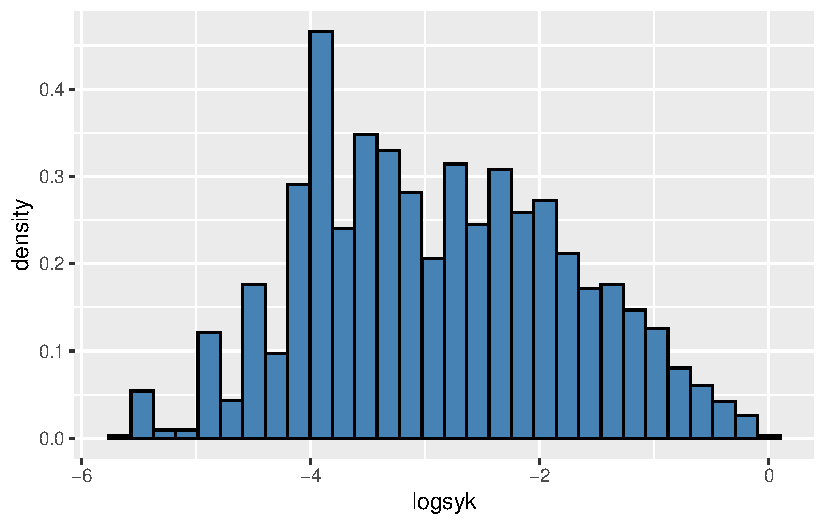
\includegraphics{kand_SOK2209_Bacheloroppgave_V25_files/figure-pdf/unnamed-chunk-18-1.pdf}

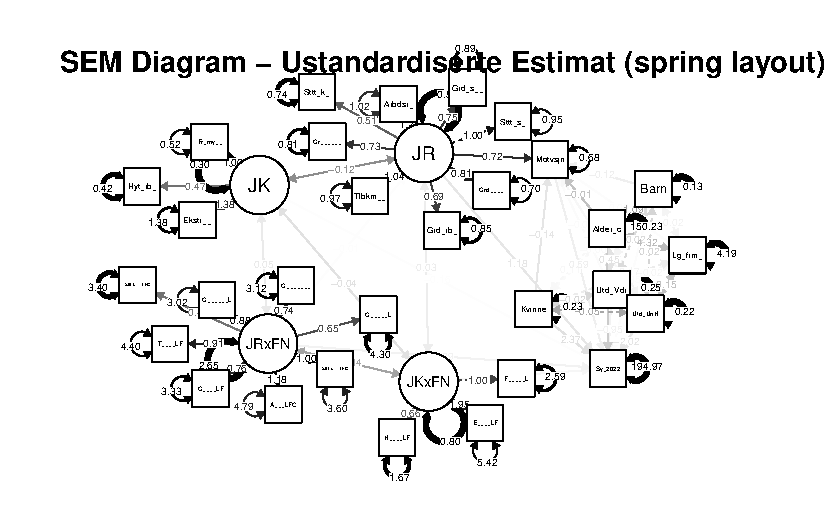
\includegraphics{kand_SOK2209_Bacheloroppgave_V25_files/figure-pdf/unnamed-chunk-18-2.pdf}

\subsubsection{Tabell med resultat fra
regresjonsanalysen(e)}\label{tabell-med-resultat-fra-regresjonsanalysene}

\subsubsection{Redegjørelse for resultat knyttet til
hypoteser}\label{redegjuxf8relse-for-resultat-knyttet-til-hypoteser}

\subsubsection{Redegjørelse for effekt av
kontrollvariabler}\label{redegjuxf8relse-for-effekt-av-kontrollvariabler}

\subsubsection{Redegjørelse for svakheter i
modellen/data}\label{redegjuxf8relse-for-svakheter-i-modellendata}

\newpage

\section{Resultat}\label{resultat}

Her presenteres den empiriske analysen og dens resultater. Vanligvis vil
en empirisk analyse bestå av en regresjonsanalyse med flere variabler.
Andre muligheter kan diskuteres med veilederen.

\subsection{Tabeller}\label{tabeller}

\subsection{Figurer}\label{figurer}

\subsection{Forklaring av tabeller og
figurer}\label{forklaring-av-tabeller-og-figurer}

\newpage

\section{Diskusjon}\label{diskusjon}

Vi tror at formue potensielt har effekt på avtalte timer også, som da
vil ha en effekt på sykefravær siden avtalte timer er endret. Men at
dette er en mer kompleks sammenheng som vi ikke har undersøkt utenom
inkludering som kontrollvariabel. Dette er en svakhet med modellen

I \autoref{sec-formue-jdr} forteller vi at effekten av formue på
sykefravær kan være ikke-lineær, og at det kan være en bueformet
sammenheng. Dette er ikke fanget opp i H1-H6 hvor vi antar lineære
interaksjoner som er en begrensning i modellen.

\paragraph{får se om vi beholder
dette}\label{fuxe5r-se-om-vi-beholder-dette}

Karrierevalg og utdanning fra gallup som viste en fattigere har
dårligere tilgang på ``career role models'' som gjør at de kanskje ikke
vet om de bedre yrkene og sånt og dermed igjen blir mindre utdanna og
sånt https://www.gallup.com/analytics/506696/amazon-research-hub.aspx så
effekt på karriærevalg, utdanning osv. langsiktig effekt av
formue/bakrunn er noe påvirker hvilken type jobb folk har og dermed
jobbkrav og jobbresssurser. Dette er da en indirekte effekt som vi ikke
får med.

Dette kapitlet drøfter resultatene i forhold til problemstillingen. Hva
er funnet ut av, hva gjenstår, hvilke styrker og svakheter har analysen?

\subsubsection{Oppsummering av hva formålet med oppgaven var, og hva
analysen
viste}\label{oppsummering-av-hva-formuxe5let-med-oppgaven-var-og-hva-analysen-viste}

\subsubsection{Diskusjon av hvilke konklusjoner som kan trekkes fra
dette og om resultatene er forenlig med tidligere
funn/teori}\label{diskusjon-av-hvilke-konklusjoner-som-kan-trekkes-fra-dette-og-om-resultatene-er-forenlig-med-tidligere-funnteori}

\subsubsection{Diskusjon av svakheter i
analysen}\label{diskusjon-av-svakheter-i-analysen}

\subsubsection{Diskusjon av implikasjoner for policy gitt
svakheter}\label{diskusjon-av-implikasjoner-for-policy-gitt-svakheter}

\subsubsection{Eventuelt: diskusjon av hva framtidig forskning kan
forske videre på (basert påderes funn og svakheter i
analysen)}\label{eventuelt-diskusjon-av-hva-framtidig-forskning-kan-forske-videre-puxe5-basert-puxe5deres-funn-og-svakheter-i-analysen}

\newpage

\section*{Referanser}\label{referanser}

\newpage

\section*{Vedlegg}\label{vedlegg}

Her legger vi til vår QMD fil.

\section*{Appendiks}\label{appendiks}

\subsection*{Kode}\label{kode}

\subsection*{Tester}\label{tester}

\subsection*{Kunstig intelligens}\label{kunstig-intelligens}

\section{notater}\label{notater}

er det avvik mellom fastsatt arbeidstid og hvor mye folk arbeider?

Er folk overarbeidet?

https://www.dagensperspektiv.no/synspunkt/benedicte-langseth-eide-svarer-hr-norge-om-sykefravaer-og-ledelse/1262876

https://www.nord24.no/nar-bedriftene-sliter-med-hoyt-sykefravar-ringer-de-benedicte-disse-tiltakene-nytter/s/5-32-197683

https://www.mdpi.com/1660-4601/18/8/4327

The results provide longitudinal evidence that two well-established job
resources (i.e., social support and feedback) predicted work engagement,
that work engagement was negatively related to sick leave and that this
relation was mediated by subjective health. By showing that
health-related indicators could also be outcomes of the motivational
process in the JD-R model, we have strengthened the model.

https://munin.uit.no/handle/10037/15801

The results also revealed that both workaholics and work-engaged
employees put in more hours at work than was expected of them. We found
that workaholism was negatively related to work-related health, whereas
work engagement was positively related to work-related health. These
findings support the notion of workaholism and work engagement as two
different forms of working hard.

Kanskje en form for ``intensitet'' i hvor sensitiv du er.

Jeg tror formue spiller inn til hvor sensitiv du er til endringer i
inntekt. Altså ditt konsumnnivå eller etterspurt fritid endrer seg ulikt
basert på om du har mye formue eller ikke. Dette kan være fordi du har
mer buffer til å tåle endringer i inntekt.

trur vi blir å få noe bue på den effekten. fattige, vanlige, rike,
megarike vil ha ulik effekt av motivasjon og sånt. e du megarik så har
det jo ingenting og si, e du syk eller vil ta fri så blir du hjemme, men
samtidig så vil du kanskje være spesielt sensitiv om du e fattig og at
om du da e syk eller vil ta fri så vil du både ha dårligere utgangspunkt
i jobbtype og sånt, og også kunne rett å slett være mer syk

mens de i midten rundt ``vanlige'' mot bare rike kan ha 0 effekt, men
kommer vel an på kor mye man ska mene formue har å si til hvor sensitiv
du er til endringer eller potentielle endringer i inntekt derfor æ
tenkte å bare ha det til å være en funksjon av formue kunne være enklere
motivasjon og sånt altså både på bunn og på topp så vil du også ha økt
den stygge m'en ved at du får statlige overføringe som fattig men mye
kapitalfortjeneste som rik

så formue har effekt på hvor mye utdanning du har. formue har effekt på
hvilken motivasjon du har. formue har effekt på m som er annen inntekt
utenom jobb.

g = formue, j = alder, k = utdanning, l = motivasjon

\begin{itemize}
\tightlist
\item
  v = dummyvariabel
\end{itemize}

\[
t^a = h^* - \alpha w - \beta(m(g) + h^*w) - (k\cdot v+j\cdot v)
\]

Dummy variabler for ulike aldersgrupper. beholde en ligning for alle men
da bruke de dummyvariablene. dermed kunne tolke bare en variabel.

forskjellige typer inntekt påvirke forskjellig i m variabelen.

Grunn til cb er at den er enkel og at vi nesten alltid tar log av
dataen. om vi har 0 variabler så blir det bare tull.

\subsubsection{Motivasjonseffekt av
ulikhet}\label{motivasjonseffekt-av-ulikhet}

``The motivational cost of inequality: Opportunity gaps reduce the
willingness to work'' https://pmc.ncbi.nlm.nih.gov/articles/PMC7473543/

https://www.brookings.edu/articles/income-inequality-social-mobility-and-the-decision-to-drop-out-of-high-school/

ulikhet gjør at fattige blir mindre motivert siden dem føler det å bli
rik er ``umulig'' og dermed investerer mindre i seg -\textgreater{}
lavere motivasjon og lavere utdanning. kanskje mer fysisk arbeid.

\subsection{Notater}\label{notater-1}

Har høy/lav formue effekt på motivasjonen fra lønnen til arbeid. lav
formue + høy lønn = høy motivasjon? høy formue + høy lønn = ``bryr meg
ikke'' = høy formue+ lav lønn, lav formue + lav lønn = lav motivajon

Kapitalinntekter som rente/aksje osv i forhold til bruttofinanskapital i
alt. kan det være at de med høy formue utenom bolig da har mer andre
inntekter, eller at høy formue bare er lik bolig for mange.

\subsubsection{Formueeffekt på konsum}\label{formueeffekt-puxe5-konsum}

https://fnce.wharton.upenn.edu/wp-content/uploads/2019/08/chodorowreich-crns\_stock\_wealth\_effects.pdf

for hver dollar i formue du har så har du 0.028usd mer i konsum eller
noe

https://usa.visa.com/partner-with-us/visa-consulting-analytics/economic-insights/the-sudden-increase-in-the-wealth-effect-and-its-impact-on-spending.html

så vi kan vise til hvordan de med lav formue da kan være tvungen til å
ta mer tima selv med lav motivasjon for samme konsumnivå fant det
tilfeldigvis her
https://www.economist.com/finance-and-economics/2025/03/19/the-trump-administration-is-playing-a-dangerous-stockmarket-game

\phantomsection\label{refs}
\begin{CSLReferences}{1}{0}
\bibitem[\citeproctext]{ref-demerouti2001job}
Demerouti, E., Bakker, A. B., Nachreiner, F. \& Schaufeli, W. B. (2001).
The job demands-resources model of burnout. \emph{Journal of Applied
Psychology}, \emph{86}(3), 499.

\bibitem[\citeproctext]{ref-durlauf_2022_the}
Durlauf, S. N., Kourtellos, A. \& Tan, C. M. (2022). The great gatsby
curve. \emph{Annual Review of Economics}, \emph{14}.
\url{https://doi.org/10.1146/annurev-economics-082321-122703}

\bibitem[\citeproctext]{ref-cfpbconsumerfinancialprotectionbureau_2015_financial}
Financial Protection Bureau), C. (Consumer. (2015). \emph{Financial
well-being: The goal of financial education}.
https://www.consumerfinance.gov/.
\url{https://files.consumerfinance.gov/f/201501_cfpb_report_financial-well-being.pdf}

\bibitem[\citeproctext]{ref-gesiarz2020motivational}
Gesiarz, F., De Neve, J.-E. \& Sharot, T. (2020). The motivational cost
of inequality: Opportunity gaps reduce the willingness to work.
\emph{Plos One}, \emph{15}(9), e0237914.

\bibitem[\citeproctext]{ref-hattrem_hvor}
Hattrem, A. (n.d.). \emph{Hvor mange er fattige i norge?} SSB. Retrieved
May 23, 2025, from
\url{https://www.ssb.no/inntekt-og-forbruk/inntekt-og-formue/artikler/hvor-mange-er-fattige-i-norge}

\bibitem[\citeproctext]{ref-hobfoll1989conservation}
Hobfoll, S. E. (1989). Conservation of resources: A new attempt at
conceptualizing stress. \emph{American Psychologist}, \emph{44}(3), 513.

\bibitem[\citeproctext]{ref-jaeggi2021wealth}
Jaeggi, A. V., Blackwell, A. D., Von Rueden, C., Trumble, B. C.,
Stieglitz, J., Garcia, A. R., Kraft, T. S., Beheim, B. A., Hooper, P.
L., Kaplan, H., et al. (2021). Do wealth and inequality associate with
health in a small-scale subsistence society? \emph{Elife}, \emph{10},
e59437.

\bibitem[\citeproctext]{ref-langseth2021ticket}
Langseth-Eide, B. \& Vittersø, J. (2021). Ticket to ride: A longitudinal
journey to health and work-attendance in the jd-r model.
\emph{International Journal of Environmental Research and Public
Health}, \emph{18}(8), 4327.

\bibitem[\citeproctext]{ref-normann_2009_inntektsfattig}
Normann, T. M. (2009). \emph{Inntektsfattig eller levekårsfattig?}
ssb.no.
\url{https://www.ssb.no/sosiale-forhold-og-kriminalitet/artikler-og-publikasjoner/inntektsfattig-eller-levekaarsfattig}

\bibitem[\citeproctext]{ref-pickett2015income}
Pickett, K. E. \& Wilkinson, R. G. (2015). Income inequality and health:
A causal review. \emph{Social Science \& Medicine}, \emph{128},
316--326.

\bibitem[\citeproctext]{ref-JSSv048i02}
Rosseel, Y. (2012). Lavaan: An r package for structural equation
modeling. \emph{Journal of Statistical Software}, \emph{48}(2), 1--36.
\url{https://doi.org/10.18637/jss.v048.i02}

\bibitem[\citeproctext]{ref-schaufeli2004job}
Schaufeli, W. B. \& Bakker, A. B. (2004). Job demands, job resources,
and their relationship with burnout and engagement: A multi-sample
study. \emph{Journal of Organizational Behavior: The International
Journal of Industrial, Occupational and Organizational Psychology and
Behavior}, \emph{25}(3), 293--315.

\bibitem[\citeproctext]{ref-ssb2024beregnet}
SSB. (2017). \emph{Beregnet bruttofinanskapital}.
\url{https://www.ssb.no/a/metadata/conceptvariable/vardok/3449/nb}

\bibitem[\citeproctext]{ref-unguren2021moderator}
Üngüren, E., Tekin, Ö. A., Avsallı, H. \& Kaçmaz, Y. Y. (2021). The
moderator role of financial well-being on the effect of job insecurity
and the COVID-19 anxiety on burnout: A research on hotel-sector
employees in crisis. \emph{Sustainability}, \emph{13}, 9031.
\url{https://doi.org/10.3390/su13169031}

\bibitem[\citeproctext]{ref-vander2016job}
Vander Elst, T., Cavents, C., Daneels, K., Johannik, K., Baillien, E.,
Van den Broeck, A. \& Godderis, L. (2016). Job demands--resources
predicting burnout and work engagement among belgian home health care
nurses: A cross-sectional study. \emph{Nursing Outlook}, \emph{64}(6),
542--556.

\end{CSLReferences}



\end{document}
